% =====================================================================
%  ch04.tex —— 第 4 章 基础同伦论（原书 p.45–73）
%  §4.1 同伦群的定义  §4.2 同伦群的基本性质  §4.3 关于 π_n(S^m) 的事实
%  §4.4 纤维丛同伦群的长正合列（4.4.1 陈述 / 4.4.2 用例 / 4.4.3 证明思路）
%  §4.5 李群的同伦群  §4.6 球面上的主丛（4.6.1 一般性 / 4.6.2 例 / 4.6.3 再谈长正合列）
%  §4.7 拓扑孤子与同伦群（4.7.1 无芯孤子（织构）/ 4.7.2 有芯孤子（拓扑缺陷））
%  注意：p.45 顶部为第 3 章 §3.7 末尾（式 3.57 及一句话），按整页切块归入本 chunk，
%        故 \chapter 出现在 p.45 中段，与原书版式一致。
%  本章共 73 个灰框编号陈述（4.1–4.73，含 5 个「事实」与 2 个「附注」）。
% =====================================================================

% [原文 p.45]
\chapter{基础同伦论}

下面进入真正的代数拓扑。

\section{同伦群的定义}

% [原文 p.46]
\begin{center}
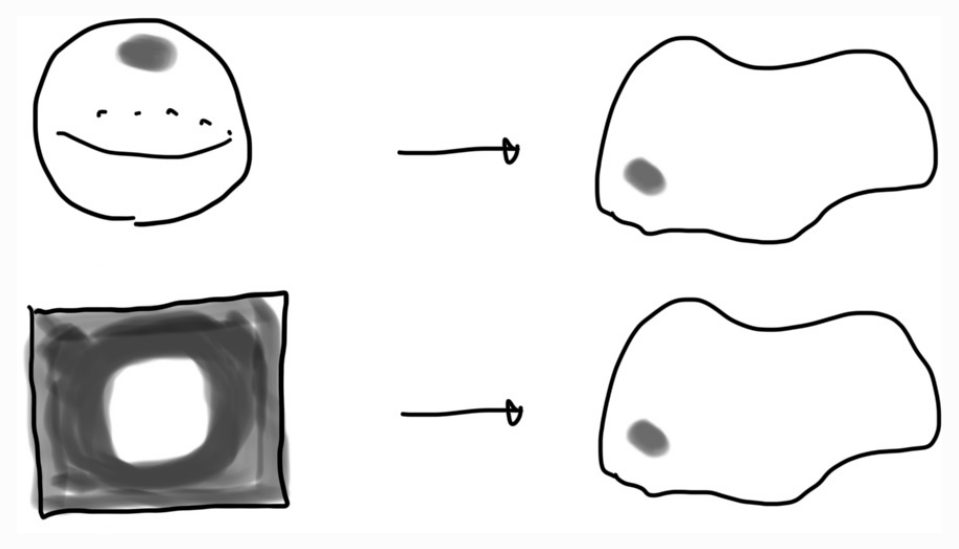
\includegraphics[width=0.62\textwidth]{figures/fig4_1.png}\\*[2pt]
{\small 图 4.1：把 $f\in[S^n,X]_\ast$ 看作从 $[0,1]^n$ 到 $X$ 的映射。阴影区域被映到基点 $\ast\in X$。}
\end{center}

\begin{definition}{4.1}
拓扑空间之间的两个映射 $f,g:X\to Y$ 称为同伦的（homotopic），若存在连续映射 $F:X\times[0,1]\to Y$，使得对一切 $x\in X$ 有 $F(x,0)=f(x)$、$F(x,1)=g(x)$。$F$ 称为 $f$ 与 $g$ 之间的同伦（homotopy）。
\end{definition}

取 $s\in[0,1]$，则 $F_s(x):=F(x,s)$ 是映射 $X\to Y$。上面的条件意味着 $F_0=f$、$F_1=g$。因此 $F_s$ 给出从 $f$ 到 $g$ 的连续形变。

在 §2.7 中，我曾对光滑映射与连续映射、光滑流形与拓扑流形的区别大做文章。对于光滑流形的同伦论，我们通常不必为这个区别操心，因为有以下事实。

\begin{qmbox}\qmstmt{事实}{4.2}
光滑流形之间的任何连续映射都同伦于一个光滑映射。
\end{qmbox}

当然，如果我们想研究光滑与连续这个问题本身，那它还是有关系的。

继续。

\begin{proposition}{4.3}
同伦是一种等价关系。
\end{proposition}

\begin{definition}{4.4}
映射在同伦下的等价类称为同伦类（homotopy class）。我们用 $[X,Y]$ 表示映射 $X\to Y$ 的同伦类的集合。
\end{definition}

在讲究一点的同伦论讲述中，下面这个概念必不可少：

\begin{definition}{4.5}
拓扑空间 $X$ 与点 $p\in X$ 组成的对 $(X,p)$ 称为带基点的空间（pointed space），$p$ 称为基点（base point）。
\end{definition}

我们常把“带基点的空间 $(X,p)$”简写成“带基点的空间 $X$”。此外，当 $X$ 连通时，$p\in X$ 的选取通常无关紧要。为此，在这种情形下我们常用记号 $\ast$ 表示基点。

\begin{definition}{4.6}
带基点空间之间的映射 $f:(X,p)\to(Y,q)$ 若满足 $f(p)=q$，则称为带基点的映射（pointed map）。
\end{definition}

我们可以像定义映射的同伦那样，定义带基点映射的同伦。

\begin{definition}{4.7}
对带基点空间 $X,Y$，我们用 $[X,Y]_\ast$ 表示带基点映射 $X\to Y$ 的同伦类的集合。
\end{definition}

我们把 $S^n$ 看作以北极点为基点的带基点空间。以下总设 $n\ge1$。现在，对带基点空间 $(X,\ast)$，考虑 $f\in[S^n,X]_\ast$。这样的 $f$ 决定一个从 $n$ 维立方体到 $X$ 的映射
\begin{equation}
f:[0,1]^n\to X
\tag{4.1}
\end{equation}
使得立方体边界的一个邻域被映到基点 $\ast\in X$，见图 4.1。

我们可以在 $[S^n,X]_\ast$ 上定义群运算如下。取 $f,g\in[S^n,X]_\ast$，把它们看作映射 $f,g:[0,1]^n\to X$。然后由下式定义 $fg:[0,1]^n\to X$：
\begin{equation}
(fg)(x_1,\dots,x_n)=
\begin{cases}
f(2x_1,x_2,\dots,x_n) & \text{当 } x_1\in[0,1/2],\\
g(2x_1-1,x_2,\dots,x_n) & \text{当 } x_1\in[1/2,1],
\end{cases}
\tag{4.2}
\end{equation}
见图 4.2。

我们再定义 $f^{-1}$ 为
\begin{equation}
f^{-1}(x_1,\dots,x_n)=f(1-x_1,x_2,\dots,x_n).
\tag{4.3}
\end{equation}
作为单位元，我们取把整个 $S^n$ 映到基点 $\ast\in X$ 的映射 $e:S^n\to X$。

% [原文 p.47]
\begin{center}
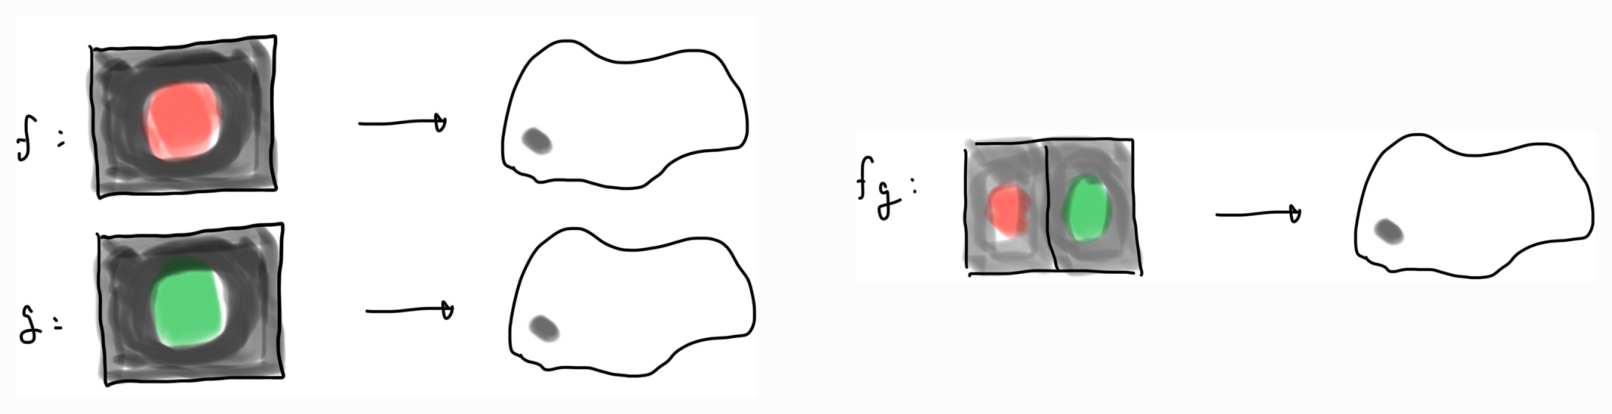
\includegraphics[width=0.62\textwidth]{figures/fig4_2.png}\\*[2pt]
{\small 图 4.2：$[S^n,X]_\ast$ 上的群运算 $fg$。阴影区域被映到基点 $\ast\in X$。}
\end{center}

\begin{proposition}{4.8}
带上述群运算的集合 $[S^n,X]_\ast$（$n\ge1$）是一个群。
\end{proposition}

\begin{definition}{4.9}
群 $[S^n,X]_\ast$（$n\ge1$）称为 $X$ 的第 $n$ 个同伦群，记作 $\pi_n(X)$。
\end{definition}

当 $n=1$ 时，$\pi_1(X)$ 也称为 $X$ 的基本群。它是从基点到基点的闭道路构成的群，群运算由道路的连接给出。

\begin{example}{4.10}
$\pi_n(\pt)=0$，其中 $\pt$ 表示单点空间。
\end{example}

\begin{example}{4.11}
$\pi_n(\R^k)=0$。
\end{example}

\begin{example}{4.12}
$\pi_1(S^1)=[S^1,S^1]_\ast=\Z$。
\end{example}

这是因为，当我们沿源 $S^1$ 绕一圈时，$f$ 的像绕目标 $S^1$ 转多少圈，就完全决定了 $f:S^1\to S^1$。这个数在物理文献中称为缠绕数（winding number），数学家则称之为映射的度（degree）。图 4.3 是一个图示。

如图所示，要让这个概念更精确，可以这样做：在目标 $S^1$ 中取一个一般位置的点 $p$，考虑它的原像 $f^{-1}(p)$。一般说来，它由源 $S^1$ 中的有限多个点组成。我们按 $f$ 在每个点处的局部定向给这些点加权，然后计数。可以证明这个数不依赖于目标 $S^1$ 中点 $p$ 的选取，从而给出缠绕数的一个定义。在图 4.3 中，$p$ 的原像由一个点组成，给出缠绕数 $+1$；相反，$q$ 的原像由三个点组成，局部定向依次为 $+1,-1,+1$，同样给出缠绕数 $+1-1+1=+1$。

% [原文 p.48]
\begin{center}
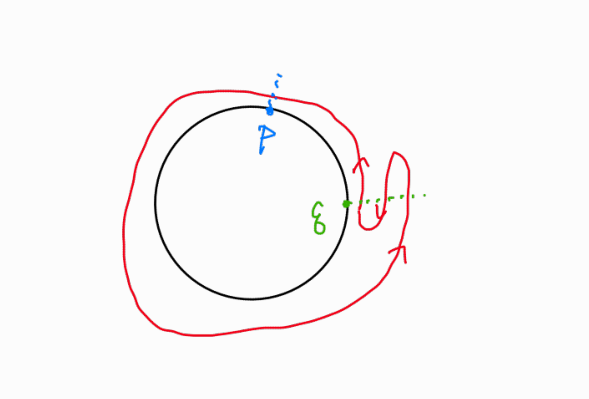
\includegraphics[width=0.34\textwidth]{figures/fig4_3.png}\\*[2pt]
{\small 图 4.3：映射 $f:S^1\to S^1$ 的缠绕数。}
\end{center}

\begin{example}{4.13}
对亏格为 $g$ 的曲面 $\Sigma_g$，
\begin{equation}
\begin{aligned}
\pi_1(\Sigma_g)=\big\langle &A_1,B_1,A_2,B_2,\dots,A_g,B_g \mid\\
&A_1B_1A_1^{-1}B_1^{-1}A_2B_2A_2^{-1}B_2^{-1}\cdots A_gB_gA_g^{-1}B_g^{-1}\big\rangle.
\end{aligned}
\tag{4.4}
\end{equation}
\end{example}

这里 $A_i$ 与 $B_i$ 是以基点为起点和终点的闭道路，它们以两种方式绕过第 $i$ 个洞，见图 4.4。右端的记号 $\langle a,b,\dots\mid \text{关系}_1,\text{关系}_2,\dots\rangle$ 称为群的一个展示（presentation）。

\begin{center}
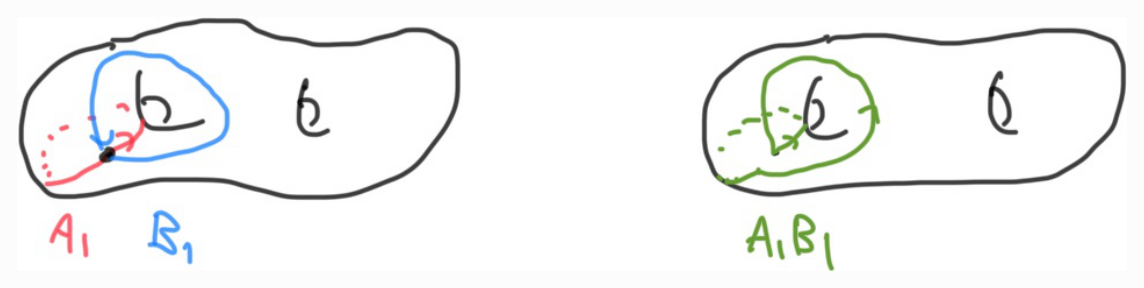
\includegraphics[width=0.62\textwidth]{figures/fig4_4.png}\\*[2pt]
{\small 图 4.4：$\pi_1(\Sigma_2)$ 的生成元。}
\end{center}

当 $g=1$，即 $\Sigma_1=T^2$ 时，它是阿贝尔群；具体地，$\pi_1(T^2)=\Z^2$。但当 $g\ge2$ 时，它是非阿贝尔的离散群。

与此相对，我们有：

\begin{proposition}{4.14}
当 $n\ge2$ 时，群 $\pi_n(X)$ 是阿贝尔的。
\end{proposition}

证明见图 4.5。要点在于，我们可以利用 $[0,1]^n$ 中 $f$ 与 $g$ 都被映到基点的那块大区域，让映射 $f$ 与 $g$ 的非平凡部分连续地互相穿过。这只有在 $n\ge2$ 时才可能。

有时定义下面这个东西也很有用：

\begin{definition}{4.15}
我们定义 $\pi_0(X)$ 为 $[S^0,X]_\ast$。它是 $X$ 的连通分支的集合。
\end{definition}

% [原文 p.49]
\begin{center}
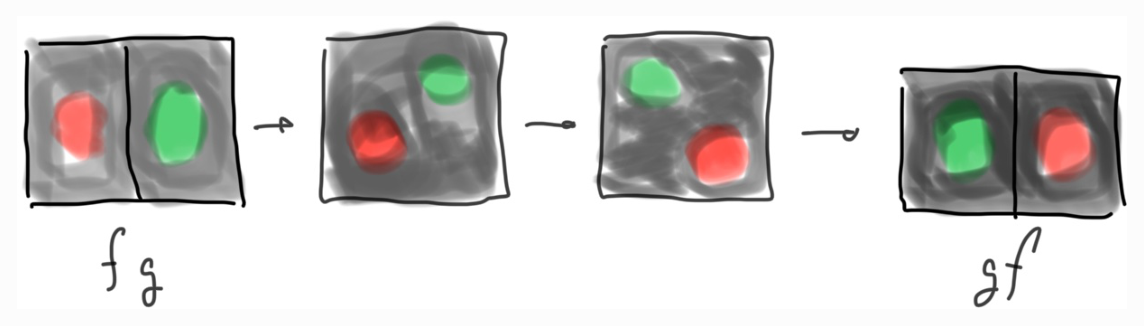
\includegraphics[width=0.62\textwidth]{figures/fig4_5.png}\\*[2pt]
{\small 图 4.5：当 $n\ge2$ 时 $\pi_n(X)$ 中群运算的交换性。}
\end{center}

的确，$S^0=\{\ast,p\}$，其中 $\ast$ 是基点。于是 $f:S^0\to X$ 由 $f(p)\in X$ 决定。我们把 $f$ 模去同伦来看，这意味着 $f$ 由 $f(p)$ 所在的 $X$ 的连通分支决定。

把到目前为止的讨论总结一下：

\begin{itemize}
  \item $\pi_0(X)$ 是一个集合。
  \item $\pi_1(X)$ 是一个群，又称 $X$ 的基本群。
  \item $\pi_{n\ge2}(X)$ 是一个阿贝尔群。
\end{itemize}

下面这个概念后来被证明很有用：

\begin{definition}{4.16}
若 $\pi_0(X)=0$，则空间 $X$ 称为连通的；若 $\pi_{0,1}(X)=0$，则称为单连通的。更一般地，若 $\pi_{0,\dots,n}(X)=0$，则空间 $X$ 称为 $n$-连通的。
\end{definition}

特别地，0-连通就是连通，1-连通就是单连通。

\takeaway{同伦是映射之间的一族连续形变，它把映射分成同伦类。带基点映射的同伦类 $\pi_n(X)$ 对 $n\ge1$ 构成群：$\pi_1$ 是基本群，$n\ge2$ 时是阿贝尔群；$\pi_0$ 只是连通分支的集合。}

\section{同伦群的基本性质}

\begin{definition}{4.17}
对映射 $f:X\to Y$ 与 $a:S^n\to X$，我们有映射 $f\circ a:S^n\to Y$。这决定了一个映射 $\pi_n(X)\to\pi_n(Y)$，容易看出它是同态。
\end{definition}

\begin{proposition}{4.18}
若两个映射 $f,g:X\to Y$ 同伦，则相应的同态 $f_\ast,g_\ast:\pi_n(X)\to\pi_n(Y)$ 相同。
\end{proposition}

特别地，若 $f:X\to X$ 同伦于恒等映射，则 $f_\ast:\pi_n(X)\to\pi_n(X)$ 是同构。这促使我们引入下面的定义：

\begin{definition}{4.19}
若存在映射 $f:X\to Y$ 与 $g:Y\to X$，使得 $f\circ g$ 同伦于 $\id_Y$、$g\circ f$ 同伦于 $\id_X$，则称两个空间 $X$ 与 $Y$ 同伦等价（homotopy equivalent）。
\end{definition}

于是有以下结论：

% [原文 p.50]
\begin{proposition}{4.20}
若 $f:X\to Y$ 给出同伦等价，则 $f_\ast:\pi_n(X)\to\pi_n(Y)$ 是同构。
\end{proposition}

当 $X$ 与 $Y$ 同胚时，即存在一一连续映射 $f:X\to Y$ 时，取 $g=f^{-1}$ 便知 $X$ 与 $Y$ 同伦等价。但 $X$ 与 $Y$ 同伦等价这个条件要宽松得多。

\begin{example}{4.21}
圆盘 $D^2=\{|x|^2+|y|^2\le1\}$ 同伦等价于一点。
\end{example}

的确，令 $f:D^2\to\{(0,0)\}$ 为显然的映射，$g:\{(0,0)\}\to D^2$ 为包含映射。$f\circ g$ 是恒等映射。所以只需证明 $g\circ f$ 同伦于恒等映射。为此，对 $s\in[0,1]$ 考虑 $f_s((x,y))=s(x,y)$，就完成了。类似地，

\begin{example}{4.22}
任意维数的圆盘 $D^n$ 都同伦等价于一点。
\end{example}

因此，若能对某个 $n$ 算出 $\pi_n(X)$ 与 $\pi_n(Y)$，并证明 $\pi_n(X)\ne\pi_n(Y)$，那么 $X$ 与 $Y$ 在这个非常宽松的等价关系下也不等价。特别地，$X$ 与 $Y$ 既不同胚也不同微分同胚。同伦群 $\pi_n(X)$ 就是这样帮助区分空间的。可是我们还没学会怎么计算同伦群。而这件事难得出奇！

为了找点感觉，我们再列举一些性质：

\begin{proposition}{4.23}
$\pi_n(X\times Y)=\pi_n(X)\times\pi_n(Y)$。
\end{proposition}

由此可以把乘积流形的同伦群计算归结为各因子的同伦群。

\begin{proposition}{4.24}
若 $X$ 是流形，则 $\pi_n(X)$ 是有限生成群。
\end{proposition}

特别地，$\pi_n(X)$ 不可能是像 $U(N)$ 那样的连续群。

有限生成阿贝尔群的结构如下：

\begin{qmbox}\qmstmt{事实}{4.25}
有限生成阿贝尔群 $A$ 都具有形式
\begin{equation}
A=\Z^n\oplus\Z_{m_1}\oplus\cdots\oplus\Z_{m_k}.
\tag{4.5}
\end{equation}
\end{qmbox}

\begin{definition}{4.26}
在上述分解中，$\Z^n$ 称为 $A$ 的自由部分，$\Z_{m_1}\oplus\cdots\oplus\Z_{m_k}$ 称为 $A$ 的挠部分。
\end{definition}

因此，当 $n\ge2$ 时，流形 $X$ 的 $\pi_n(X)$ 总具有式 (4.5) 的形式。

\takeaway{同伦群对同伦等价不变：同胚或同伦等价的映射诱导同构，可缩空间的所有同伦群都平凡。乘积空间的同伦群是各因子的直积；紧流形的同伦群有限生成，可分解为自由部分与挠部分。}

\section{关于 $\pi_n(S^m)$ 的事实}

我们来看看同伦群的具体例子。作为开始，先考虑球面自身的同伦群，即 $\pi_n(S^m)=[S^n,S^m]_\ast$。

% [原文 p.51]
\begin{center}
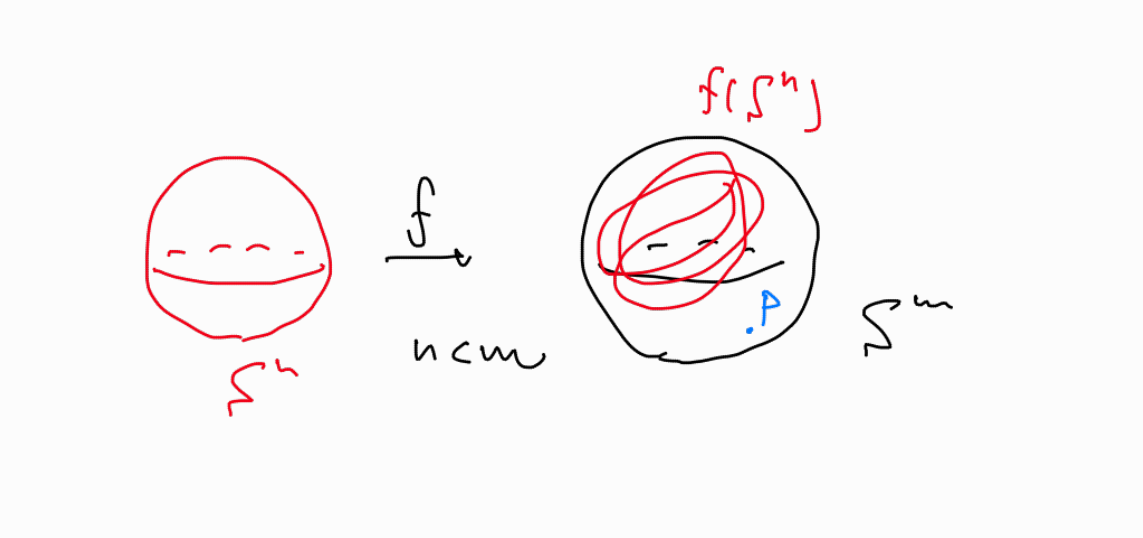
\includegraphics[width=0.62\textwidth]{figures/fig4_6.png}\\*[2pt]
{\small 图 4.6：当 $n<m$ 时，一般位置的映射 $S^n\to S^m$ 会留下一个点 $p\in S^m$ 不被 $S^n$ 映到。}
\end{center}

\begin{theorem}{4.27}
若 $n<m$，则 $\pi_n(S^m)=0$。
\end{theorem}

粗略地说，当 $n<m$ 时，一般位置的映射 $S^n\to S^m$ 会漏掉某个点 $p\in S^m$，即 $p$ 不在 $S^n$ 的像中。我们可以把映射的像从该点“推”向基点。因此每个映射都同伦于把 $S^n$ 映到基点的映射，见图 4.6。

\begin{theorem}{4.28}
$\pi_n(S^n)=\Z$。
\end{theorem}

这可以通过考虑缠绕数的高维版本来证明。对映射 $f:S^n\to S^n$，得到的整数在数学中称为它的度（degree）。

更有趣的是下面这个：

\begin{theorem}{4.29}
$\pi_3(S^2)=\Z$。此外，Hopf 纤维化 $S^3\to S^2$ 对应 $\Z$ 的生成元。
\end{theorem}

给定映射 $f:S^3\to S^2$，相应的整数这样得到。在 $S^2$ 上取一个一般位置的点 $p$，其原像 $f^{-1}(p)$ 是 $S^3$ 中的一族圆周 $C_1,\dots,C_n$。再在 $S^2$ 上取另一个点 $q$，其原像 $f^{-1}(q)$ 是 $S^3$ 中的另一族圆周 $C'_1,\dots,C'_m$。现在我们考虑
\begin{equation}
\sum_{i,j}\mathrm{Lk}(C_i,C'_j),
\tag{4.6}
\end{equation}
其中两个圆周的环绕数 $\mathrm{Lk}$ 按通常方式定义。\footnote[11]{这出现在电磁学方程的积分形式中。具体地说，若有电流 $I$ 沿环路 $C$ 流动，则 $C'$ 周围的磁场积分正比于 $C$ 与 $C'$ 的环绕数。}可以证明，它在 $f$ 的连续形变下不变。这是 $f$ 的 Hopf 不变量的一种定义。定义的图示见图 4.7。

我们已在图 3.3 中画过 Hopf 纤维化 $S^1\to S^3\to S^2$ 的实际纤维。观察可知，两条纤维的环绕数为 1。因此，Hopf 纤维化 $S^3\to S^2$ 的 Hopf 不变量为 1。

% [原文 p.52]
\begin{center}
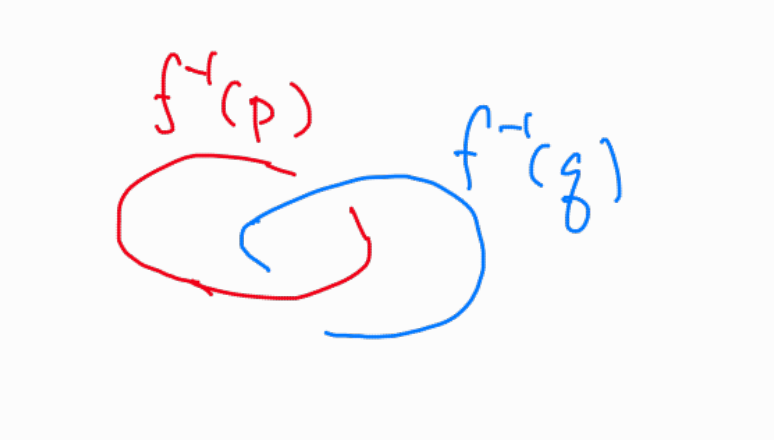
\includegraphics[width=0.42\textwidth]{figures/fig4_7.png}\\*[2pt]
{\small 图 4.7：映射 $f:S^3\to S^2$ 的 Hopf 不变量的一种定义：考虑 $S^2$ 中两点的原像的环绕数。}
\end{center}

我们可以类似地定义 $S^{2n-1}$ 中两个 $S^{n-1}$ 的环绕数（$n>2$），先前的讨论对应 $n=2$ 的情形。于是，对映射 $f:S^{2n-1}\to S^n$，$S^n$ 中一般位置点的原像是一个 $(n-1)$ 维空间，我们就可以像式 (4.6) 那样定义 $f$ 的高维 Hopf 不变量。现在已知，一般地有
\begin{equation}
\mathrm{Lk}(A,B)=(-1)^n\,\mathrm{Lk}(B,A)
\tag{4.7}
\end{equation}
这意味着当 $n$ 为奇数时，表达式 (4.6) 给出零。正如我们将在下面命题 4.33 中看到的，当 $n$ 为偶数时，构造一个 Hopf 不变量为 2 的映射 $S^{2n-1}\to S^n$ 相对容易，因此

\begin{theorem}{4.30}
$\pi_{4m-1}(S^{2m})$ 含有一个 $\Z$ 直和项。
\end{theorem}

此外，通过显式计算可以证明

\begin{proposition}{4.31}
Hopf 纤维化 $S^3\to S^2$、$S^7\to S^4$、$S^{15}\to S^8$ 的 Hopf 不变量都为 1。
\end{proposition}

而事实上

\begin{theorem}{4.32}
只有当 $n=2,4,8$ 时，才存在 Hopf 不变量为 1 的映射 $f:S^{2n-1}\to S^n$。
\end{theorem}

这是代数拓扑中的一个深刻结果，称为 Hopf 不变量一问题；解决这个问题的努力推动了该领域的许多发展。我们还有

\begin{proposition}{4.33}
对其余所有 $n=2m$，映射 $f:S^{4m-1}\to S^{2m}$ 的最小 Hopf 不变量为 2。
\end{proposition}

\begin{proof}[证明思路]
这可以通过用 Whitehead 积构造一个 Hopf 不变量为 2 的例子来证明。这里我们没有时间给出一般理论，所以直接给出最终构造出的映射。

% [原文 p.53]
暂且设 $n$ 为任意整数，不假定它为偶数。首先，把 $S^{2n-1}$ 实现为
\begin{equation}
(S^{n-1}\times D^n)\cup(D^n\times S^{n-1}),
\tag{4.8}
\end{equation}
其中把公共边界 $S^{n-1}\times S^{n-1}$ 按适当的定向粘合。然后，利用把边界缩到基点的映射 $g:D^n\to S^n$，如下定义映射 $f:S^{2n-1}\to S^n$：
\begin{equation}
f(p)=
\begin{cases}
g(b) & \text{若 } p=(a,b)\in S^{n-1}\times D^n,\\
g(a) & \text{若 } p=(a,b)\in D^n\times S^{n-1}.
\end{cases}
\tag{4.9}
\end{equation}
于是，对远离基点的一般位置的点 $s\in S^{n-1}$，其原像 $f^{-1}(s)$ 为
\begin{equation}
f^{-1}(s)=(\{s\}\times S^{n-1})\cup(S^{n-1}\times\{s\}),
\tag{4.10}
\end{equation}
现在有
\begin{align}
\mathrm{Lk}(\{s\}\times S^{n-1},\{t\}\times S^{n-1})&=0,\tag{4.11}\\
\mathrm{Lk}(\{s\}\times S^{n-1},S^{n-1}\times\{t\})&=1,\tag{4.12}
\end{align}
利用这些可以算出
\begin{equation}
\mathrm{Lk}(f^{-1}(s),f^{-1}(t))=
\begin{cases}
2 & \text{（$n$ 为偶数）},\\
0 & \text{（$n$ 为奇数）},
\end{cases}
\tag{4.13}
\end{equation}
这里用到了式 (4.7)。
\end{proof}

另一个有趣的事实是

\begin{theorem}{4.34}
$\pi_n(S^m)$ 的自由部分只可能来自 $\pi_n(S^n)\simeq\Z$ 与上面讨论过的 $\pi_{2n-1}(S^n)$ 的那个 $\Z$ 直和项。除此以外，球面的同伦群全是挠。
\end{theorem}

讲完这些基本性质，我们来看看 $n$ 与 $k$ 都较小时球面的同伦群 $\pi_{n+k}(S^n)$，它们列在表 1 中。数据取自岩波数学辞典 [日07、附录、公式 7、V]，它也有英译本 [Itö87]。在那里，我们用红色表示 $\pi_d(S^d)\simeq\Z$，用蓝色表示 $\pi_{2m-1}(S^m)$ 中的那个 $\Z$ 直和项。

表中显然还能看出更多规律。这来自下面的一般事实。我们先从一个定义开始。

\begin{definition}{4.35}
给定带基点空间 $(X,\ast)$，我们定义 $X$ 的约化悬挂 $\Sigma X$ 为
\begin{equation}
\Sigma X=\frac{X\times[0,1]}{X\times\{0,1\}\cup\{\ast\}\times[0,1]}.
\tag{4.14}
\end{equation}
\end{definition}

图示见图 4.8。

% [原文 p.54]
\begin{center}
\begin{minipage}{\linewidth}
\centering
\footnotesize
\setlength{\fboxsep}{0pt}%
\setlength{\tabcolsep}{0pt}%
\newcommand{\tabcell}[1]{\makebox[3.6em][c]{\rule[-0.3em]{0pt}{1.5em}#1}}%
\newcommand{\tabgray}[1]{\colorbox{black!8}{\makebox[3.6em][c]{\rule[-0.3em]{0pt}{1.5em}#1}}}%
\newcommand{\tablab}[1]{\makebox[2.0em][r]{\rule[-0.3em]{0pt}{1.5em}#1}}%
\newcommand{\redZ}{\textcolor{red}{\Z}}%
\newcommand{\blueZ}{\textcolor{blue}{\Z}}%
\begin{tabular}{c|*{10}{c}}
\hline
\tablab{$k$} & \tabcell{0} & \tabcell{1} & \tabcell{2} & \tabcell{3} & \tabcell{4} & \tabcell{5} & \tabcell{6} & \tabcell{7} & \tabcell{8} & \tabcell{9}\\
\hline
\tablab{$S^1$} & \tabcell{$\redZ$} & \tabcell{0} & \tabcell{0} & \tabcell{0} & \tabcell{0} & \tabcell{0} & \tabcell{0} & \tabcell{0} & \tabcell{0} & \tabcell{0}\\
\tablab{$S^2$} & \tabgray{$\redZ$} & \tabcell{$\blueZ$} & \tabcell{$\Z_2$} & \tabcell{$\Z_2$} & \tabcell{$\Z_{12}$} & \tabcell{$\Z_2$} & \tabcell{$\Z_2$} & \tabcell{$\Z_3$} & \tabcell{$\Z_{15}$} & \tabcell{$\Z_2$}\\
\tablab{$S^3$} & \tabgray{$\redZ$} & \tabgray{$\Z_2$} & \tabcell{$\Z_2$} & \tabcell{$\Z_{12}$} & \tabcell{$\Z_2$} & \tabcell{$\Z_2$} & \tabcell{$\Z_3$} & \tabcell{$\Z_{15}$} & \tabcell{$\Z_2$} & \tabcell{$(\Z_2)^2$}\\
\tablab{$S^4$} & \tabgray{$\redZ$} & \tabgray{$\Z_2$} & \tabgray{$\Z_2$} & \tabcell{$\blueZ\times\Z_{12}$} & \tabcell{$(\Z_2)^2$} & \tabcell{$(\Z_2)^2$} & \tabcell{$\Z_{24}\times\Z_3$} & \tabcell{$\Z_{15}$} & \tabcell{$\Z_2$} & \tabcell{$(\Z_2)^3$}\\
\tablab{$S^5$} & \tabgray{$\redZ$} & \tabgray{$\Z_2$} & \tabgray{$\Z_2$} & \tabgray{$\Z_{24}$} & \tabcell{$\Z_2$} & \tabcell{$\Z_2$} & \tabcell{$\Z_2$} & \tabcell{$\Z_{30}$} & \tabcell{$\Z_2$} & \tabcell{$(\Z_2)^3$}\\
\tablab{$S^6$} & \tabgray{$\redZ$} & \tabgray{$\Z_2$} & \tabgray{$\Z_2$} & \tabgray{$\Z_{24}$} & \tabgray{$0$} & \tabcell{$\blueZ$} & \tabcell{$\Z_2$} & \tabcell{$\Z_{60}$} & \tabcell{$\Z_{24}\times\Z_2$} & \tabcell{$(\Z_2)^3$}\\
\tablab{$S^7$} & \tabgray{$\redZ$} & \tabgray{$\Z_2$} & \tabgray{$\Z_2$} & \tabgray{$\Z_{24}$} & \tabgray{$0$} & \tabgray{$0$} & \tabcell{$\Z_2$} & \tabcell{$\Z_{120}$} & \tabcell{$(\Z_2)^3$} & \tabcell{$(\Z_2)^4$}\\
\tablab{$S^8$} & \tabgray{$\redZ$} & \tabgray{$\Z_2$} & \tabgray{$\Z_2$} & \tabgray{$\Z_{24}$} & \tabgray{$0$} & \tabgray{$0$} & \tabgray{$\Z_2$} & \tabcell{$\blueZ\times\Z_{120}$} & \tabcell{$(\Z_2)^4$} & \tabcell{$(\Z_2)^5$}\\
\tablab{$S^9$} & \tabgray{$\redZ$} & \tabgray{$\Z_2$} & \tabgray{$\Z_2$} & \tabgray{$\Z_{24}$} & \tabgray{$0$} & \tabgray{$0$} & \tabgray{$\Z_2$} & \tabgray{$\Z_{240}$} & \tabcell{$(\Z_2)^3$} & \tabcell{$(\Z_2)^4$}\\
\tablab{$S^{10}$} & \tabgray{$\redZ$} & \tabgray{$\Z_2$} & \tabgray{$\Z_2$} & \tabgray{$\Z_{24}$} & \tabgray{$0$} & \tabgray{$0$} & \tabgray{$\Z_2$} & \tabgray{$\Z_{240}$} & \tabgray{$(\Z_2)^2$} & \tabcell{$\blueZ\times(\Z_2)^3$}\\
\tablab{$S^{11}$} & \tabgray{$\redZ$} & \tabgray{$\Z_2$} & \tabgray{$\Z_2$} & \tabgray{$\Z_{24}$} & \tabgray{$0$} & \tabgray{$0$} & \tabgray{$\Z_2$} & \tabgray{$\Z_{240}$} & \tabgray{$(\Z_2)^2$} & \tabgray{$(\Z_2)^3$}\\
\tablab{$S^{12}$} & \tabgray{$\redZ$} & \tabgray{$\Z_2$} & \tabgray{$\Z_2$} & \tabgray{$\Z_{24}$} & \tabgray{$0$} & \tabgray{$0$} & \tabgray{$\Z_2$} & \tabgray{$\Z_{240}$} & \tabgray{$(\Z_2)^2$} & \tabgray{$(\Z_2)^3$}\\
\hline
\end{tabular}\\[2pt]
{\small 表 1：球面同伦群 $\pi_{n+k}(S^n)$}
\end{minipage}
\end{center}

\begin{proposition}{4.36}
$\Sigma S^n\simeq S^{n+1}$。
\end{proposition}

\begin{definition}{4.37}
给定 $f:X\to Y$，我们如下定义 $\Sigma f:\Sigma X\to\Sigma Y$：
\begin{equation}
(\Sigma f)([x,t])=([f(x),t]),
\tag{4.15}
\end{equation}
其中 $\Sigma X$ 中的点记作 $[x,t]$，$x\in X$、$t\in[0,1]$。这确定了一个映射
\begin{equation}
[X,Y]_\ast\to[\Sigma X,\Sigma Y]_\ast.
\tag{4.16}
\end{equation}
\end{definition}

特别地，取 $X=S^n$、$\Sigma X=S^{n+1}$，就有

\begin{center}
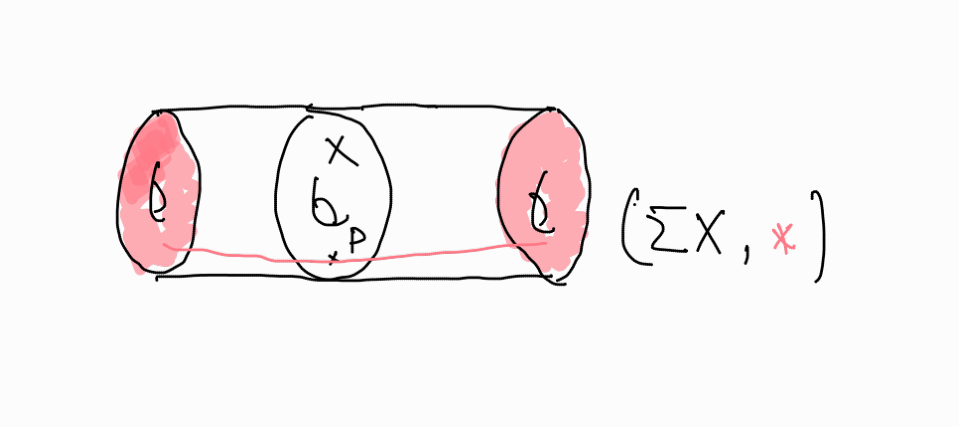
\includegraphics[width=0.62\textwidth]{figures/fig4_8.png}\\*[2pt]
{\small 图 4.8：空间 $X$ 的约化悬挂 $\Sigma X$。图中把所有染成红色的点缩为一点，取它为基点。}
\end{center}

% [原文 p.55]
\begin{proposition}{4.38}
映射 $\pi_n(Y)\to\pi_{n+1}(\Sigma Y)$ 是群同态。
\end{proposition}

此外，还有 Freudenthal 悬挂定理：

\begin{theorem}{4.39}
设 $Y$ 是 $(n-1)$-连通的，即 $\pi_{i<n}(Y)=0$。则悬挂同态 $\pi_k(Y)\to\pi_{k+1}(\Sigma Y)$ 在 $k<2n-1$ 时是同构，在 $k=2n-1$ 时是满射。
\end{theorem}

更显式地说，$\pi_{k\le n}(\Sigma Y)=0$，$\pi_k(Y)=\pi_{k+1}(\Sigma Y)$ 对 $k=0,1,\dots,2n-2$ 成立，且 $\pi_{2n-1}(Y)\to\pi_{2n}(\Sigma Y)$ 是满射。

由于 $S^n$ 显然是 $(n-1)$-连通的，特别地有

\begin{proposition}{4.40}
$\pi_{n+k}(S^n)\to\pi_{(n+1)+k}(S^{n+1})$ 在 $k<n-1$ 时是同构，在 $k=n-1$ 时是满射。
\end{proposition}

这解释了表 1 中的灰色区域。

灰色区域中的球面同伦群称为球面的稳定同伦群。更精确地说，数学家这样定义：

\begin{definition}{4.41}
我们称
\begin{equation}
\pi_k^{\mathrm{st}}:=\lim_{n\to\infty}\pi_{n+k}(S^n)
\tag{4.17}
\end{equation}
为球面的第 $k$ 个稳定同伦群，或简称第 $k$ 个 stem。
\end{definition}

相反，非灰色区域中的同伦群称为不稳定群。球面的稳定同伦群比不稳定群容易计算得多。不过，稳定同伦群还没有被完全理解。事实上，计算它们是代数拓扑的主要目标之一；目前已知到 $k\le 83$ [IWX20]。

这个领域有一个著名的原理，称为“Mahowald 不确定性原理”[IWX23, 第 3 节]：不存在一种能算出所有球面稳定同伦群的单一方法！更精确的说法是，任何收敛到 $\pi_\ast^{\mathrm{st}}$、且 $E^2$ 页有代数描述的谱序列都有无穷多个微分，因此与真正的答案相差无穷远。我希望在这套讲义中尽量多讲些背景材料，让读者至少能理解这句话。

进入下一节之前，我们先讨论稳定范围中一个与粒子物理标准模型有关的球面同伦群：

\begin{example}{4.42}
$\pi_4(S^3)=\Z_2$。
\end{example}

用 Freudenthal 悬挂定理可知，它的生成元 $S^4\to S^3$ 是 Hopf 纤维化 $p:S^3\to S^2$ 的悬挂 $\Sigma p$。但很难看出这个映射 $\Sigma p$ 生成一个 $\Z_2$，而且没有别的生成元。


% [原文 p.56]
\begin{remark}{4.43}
它在四维物理中的表现如下。弱相互作用由 $SU(2)$ 规范理论描述，因此我们的时空中有一个 $SU(2)$ 主丛。取时空的一个片 $\R^4$，就可以考虑规范变换
\begin{equation}
g:\R^4\to SU(2).
\tag{4.18}
\end{equation}
假定我们在远处区域不做任何规范变换。那么本质上就得到一个映射
\begin{equation}
g:S^4\to SU(2)\simeq S^3.
\tag{4.19}
\end{equation}
现在，我们的世界中有各种费米子。带弱相互作用荷的费米子总处在 $SU(2)$ 的双重态表示中。用 §3.7 的记号，单个双重态由 $2\otimes S\to M$ 的一个截面描述；其中 $V\to M$ 是表示 $\rho:G\curvearrowright V$ 与主 $G$-丛（principal $G$-bundle） $P\to M$ 的相伴向量丛，$S\to M$ 是旋量丛。

$SU(2)$ 的单个双重态表示中的费米子，其配分函数 $Z_{\text{single doublet}}$ 在规范变换 (4.19) 下已知会变成
\begin{equation}
Z_{\text{single doublet}}\to(-1)^sZ_{\text{single doublet}},
\tag{4.20}
\end{equation}
其中 $s=[g]\in\pi_4(S^3)\simeq\Z_2\simeq\{0,1\}$；这最早出现在 [Wit82] 中。这意味着，例如只有一个双重态的 $SU(2)$ 规范理论是不自洽的。

现在，在单代 (3.57) 中，$SU(2)$ 的双重态有 $3+1=4$ 个。因此，符号 (4.20) 总是变成 $(-1)^{4s}=+1$，理论便自洽了。举例来说，这意味着你不能只把颜色数从 $SU(3)$ 改成 $SU(4)$，而把标准模型中的其他一切都保持不变。
\end{remark}

\takeaway{同伦群 $\pi_n(S^m)$ 的算术结构由三条基本事实刻画：$n<m$ 时为零，$n=m$ 时为 $\Z$，而 $\pi_{2n-1}(S^n)$ 含一个 $\Z$ 直和项。悬挂把低维同伦群稳定地搬到高维，稳定区用灰色标出。}

\section{纤维丛同伦群的长正合列}

\subsection{陈述}

计算同伦群很难。一个有用的技巧是纤维丛 $F\to E\to B$ 对应的同伦群长正合列。它把 $\pi_\ast(F)$、$\pi_\ast(E)$ 与 $\pi_\ast(B)$ 联系起来。已知其中两个时，往往可以确定第三个。我们先从下面的定义开始：

\begin{definition}{4.44}
群与它们之间的同态构成的序列
\begin{equation}
\cdots\xrightarrow{f_{i-2}}G_{i-1}\xrightarrow{f_{i-1}}G_i\xrightarrow{f_i}G_{i+1}\xrightarrow{f_{i+1}}\cdots
\tag{4.21}
\end{equation}
若它在每个群处都正合，即对所有的 $i$ 都有 $f_{i-1}\circ f_i=0$，并且
\begin{equation}
\mathrm{Im}\,f_i=\Ker f_{i+1}\subset G_i
\tag{4.22}
\end{equation}
则称为群的正合列。
\end{definition}

这听起来可能有点晦涩，所以我们从两个较简单的情形开始。

% [原文 p.57]
\begin{proposition}{4.45}
正合列 $1\xrightarrow{f}A\xrightarrow{g}1$ 意味着 $A\simeq 1$。
\end{proposition}

为看出这一点，把条件 $\mathrm{Im}\,f=\Ker g$ 的定义展开。由于 $g$ 把一切都映到 $1$，$\Ker g$ 其实就是整个 $A$。而 $\mathrm{Im}\,f$ 只是 $\{e\}\subset A$。因此 $A=\{e\}=1$。

\begin{proposition}{4.46}
正合列 $1\xrightarrow{f}A\xrightarrow{g}B\xrightarrow{h}1$ 意味着 $A\simeq B$。
\end{proposition}

为看出这一点，展开条件 $\mathrm{Im}\,f=\Ker g$ 与 $\mathrm{Im}\,g=\Ker h$ 的定义。由于 $\mathrm{Im}\,f=\{e\}$，有 $\Ker g=\{e\}$，即 $g$ 是单射。由于 $\Ker h=B$，有 $\mathrm{Im}\,g=B$，即 $g$ 是满射。因此 $g$ 是双射，$A\simeq B$。

稍作推广便得到：

\begin{definition}{4.47}
群的正合列若具有如下形式，就称为群的短正合列：
\begin{equation}
1\to A\to B\to C\to 1.
\tag{4.23}
\end{equation}
这时称 $B$ 为 $C$ 被 $A$ 的扩张。
\end{definition}

注意，对阿贝尔群，我们常用 $0$ 而不用 $1$ 表示平凡群。

给定 $A$ 与 $C$，$B$ 并不唯一确定。例如，设涉及的群都是阿贝尔群，考虑短正合列
\begin{equation}
0\to\Z_2\to A\to\Z_2\to 0.
\tag{4.24}
\end{equation}
则 $A$ 可以是 $\Z_2\times\Z_2$ 或 $\Z_4$。在后一情形，同态由下式给出
\begin{equation}
0\to\{0,1\}\xrightarrow{\times 2}\{0,1,2,3\}\xrightarrow{\mathrm{mod}\,2}\{0,1\}\to 0.
\tag{4.25}
\end{equation}

尽管如此，短正合列仍严重限制了给定 $A$ 与 $C$ 时 $B$ 的可能。

现在，一般的正合列可以分解为短正合列：

\begin{proposition}{4.48}
群的正合列
\begin{equation}
\cdots\xrightarrow{f_{i-2}}G_{i-1}\xrightarrow{f_{i-1}}G_i\xrightarrow{f_i}G_{i+1}\xrightarrow{f_{i+1}}\cdots
\tag{4.26}
\end{equation}
给出短正合列
\begin{equation}
0\to G_{i-1}/\Ker f_{i-1}\to G_i\to\mathrm{Im}\,f_i\to 0.
\tag{4.27}
\end{equation}
\end{proposition}

这意味着，给定一个群的长正合列，我们就有了确定其中各群的许多信息。现在回到代数拓扑。

% [原文 p.58]
\begin{theorem}{4.49}
给定纤维丛
\begin{equation}
F\xrightarrow{\iota}E\xrightarrow{p}B,
\tag{4.28}
\end{equation}
就有如下同伦群的长正合列：
\begin{equation}
\begin{array}{cccccc}
\cdots & \xrightarrow{\partial} & \pi_{n+1}(F) & \xrightarrow{\iota_*} & \pi_{n+1}(E) & \xrightarrow{p_*}\pi_{n+1}(B)\\[2pt]
 & \xrightarrow{\partial} & \pi_{n}(F) & \xrightarrow{\iota_*} & \pi_{n}(E) & \xrightarrow{p_*}\pi_{n}(B)\\[2pt]
 & \xrightarrow{\partial} & \cdots & & \cdots & \\[2pt]
 & \xrightarrow{\partial} & \pi_{1}(F) & \xrightarrow{\iota_*} & \pi_{1}(E) & \xrightarrow{p_*}\pi_{1}(B)\\[2pt]
 & \xrightarrow{\partial} & \pi_{0}(F) & \xrightarrow{\iota_*} & \pi_{0}(E) & \xrightarrow{p_*}\pi_{0}(B),
\end{array}
\tag{4.29}
\end{equation}
其中最后三个对象其实不是群而是集合，但条件 (4.22) 仍然成立；映射 $\partial$ 将在下文定义 4.56 中构造。
\end{theorem}

\subsection{用例}

下面看几个基本用例。这会说明，你可以在不理解证明、甚至不理解陈述中那个重要映射 $\partial$ 的构造的情况下使用一个定理！这正是我所主张的“数学就像一套手机应用”的心态。

考虑纤维丛 $\Z\to\R\to S^1$。由于 $\pi_n(\R^k)=0$，长正合列直接给出
\begin{equation}
0=\pi_n(\R)\to\pi_n(S^1)\to\pi_{n-1}(\Z)\to\pi_{n-1}(\R)=0,
\tag{4.30}
\end{equation}
即
\begin{equation}
\pi_n(S^1)=\pi_{n-1}(\Z).
\tag{4.31}
\end{equation}
由于 $\pi_0(\Z)=\Z$、$\pi_{n\ge 1}(\Z)=0$，可得

\begin{example}{4.50}
\[
\pi_n(S^1)=\begin{cases}\Z & (n=1),\\ 0 & (n\neq 1).\end{cases}
\]
\end{example}

假设 $\Gamma$ 自由作用在 $S^n$ 上，$n\ge 2$。有纤维丛 $\Gamma\to S^n\to S^n/\Gamma$。于是有长正合列，其中一段是
\begin{equation}
\pi_1(S^n)\to\pi_1(S^n/\Gamma)\to\pi_0(\Gamma)\to\pi_0(S^n),
\tag{4.32}
\end{equation}
即
\begin{equation}
0\to\pi_1(S^n/\Gamma)\to\Gamma\to 0,
\tag{4.33}
\end{equation}
意味着 $\pi_1(S^n/\Gamma)=\Gamma$。回忆 $\RP^n=S^n/\Z_2$。因此有
\begin{equation}
\pi_1(\RP^n)=\Z_2.
\tag{4.34}
\end{equation}
再回忆一下 $SO(3)=\RP^3$。于是有

% [原文 p.59]
\begin{example}{4.51}
$\pi_1(SO(3))=\Z_2$。
\end{example}

下面把同伦群长正合列用到 Hopf 纤维化 $S^1\to S^3\to S^2$ 上。上面已经知道 $k>1$ 时 $\pi_k(S^1)=0$。因此长正合列给出
\begin{equation}
0=\pi_k(S^1)\to\pi_k(S^3)\to\pi_k(S^2)\to\pi_{k-1}(S^1)=0,
\tag{4.35}
\end{equation}
当 $k\ge 3$，即

\begin{proposition}{4.52}
对 $k\ge 3$，$\pi_k(S^3)=\pi_k(S^2)$。
\end{proposition}

这特别说明 $\pi_3(S^2)=\Z$，即我们已经提到过的基本事实，也解释了表 1 中 $S^2$ 与 $S^3$ 两列的规律。

再举一例，考虑 $\pi_1(SO(n))$ 的计算。上面刚看到 $\pi_1(SO(3))=\Z_2$。由命题 2.35 已知有纤维丛
\begin{equation}
SO(n-1)\to SO(n)\to S^{n-1}.
\tag{4.36}
\end{equation}
于是长正合列给出
\begin{equation}
\pi_2(S^{n-1})\to\pi_1(SO(n-1))\to\pi_1(SO(n))\to\pi_1(S^{n-1}).
\tag{4.37}
\end{equation}
对 $n>3$，有 $\pi_2(S^{n-1})=\pi_1(S^{n-1})=0$，因此 $\pi_1(SO(n-1))=\pi_1(SO(n))$。归纳地，就得到

\begin{example}{4.53}
对 $n\ge 3$，$\pi_1(SO(n))=\Z_2$。
\end{example}

对 $n=3$，同一长正合列的另一段给出
\begin{equation}
\begin{aligned}
&\underbrace{\pi_2(SO(2))}_{=0}\to\pi_2(SO(3))\to\underbrace{\pi_2(S^2)}_{\Z}\xrightarrow{\partial}\underbrace{\pi_1(SO(2))}_{\Z}\\
&\qquad\to\underbrace{\pi_1(SO(3))}_{=\Z_2}\ \ \pi_1(S^2)=0.
\end{aligned}
\tag{4.38}
\end{equation}
这迫使 $\partial:\Z\to\Z$ 是乘以 $2$ 的映射，于是 $\pi_2(SO(3))=0$。

\noindent\textbf{附注 4.54.}在继续之前，我们来看如何用 $\pi_1(SO(n))=\Z_2$ 这个事实说明存在非平凡同态 $\pi_4(S^3)\to\Z_2$。为此，取一个映射 $f:S^4\to S^3$，并假定它是光滑的。如同讨论 Hopf 不变量时那样，取 $S^3$ 上一个一般位置点 $p$ 的原像，它是一些不相交的圆。对每个圆 $S^1$，取一个填满它的圆盘 $D^2$。这样，通过把 $D^2\times\R^4$（$\R^4$ 中有固定的坐标架）限制到边界上，就能在 $S^1$ 的每一点处装上一个坐标架（记为 $A$）。

我们还按如下方式在 $S^1$ 的每一点处装上（可能不同的）坐标架。$S^3$ 上的点 $p$ 在 $\R^3$ 中有一个自然的坐标架。把它拉回到 $S^1\subset S^4$，就在 $S^1$ 的每一点处给出横向切片 $\R^3$ 的一个坐标架。连同 $S^1$ 的切方向，这给出另一组坐标架（记为 $B$）。两组坐标架 $A$ 与 $B$ 由一个四维旋转 $g:S^1\to SO(4)$ 相联系，它确定一个类 $\pi_1(SO(4))=\Z_2=\{\pm 1\}$。

% [原文 p.60]
回忆 $f^{-1}(p)$ 是一些不相交的圆。对每个圆按上述方式算出一个符号 $\{\pm 1\}$，再把它们乘起来。这样就从光滑映射 $f:S^4\to S^3$ 得到了一个符号 $\pm 1$。可以证明，它不依赖于所做的各种选择，也不依赖于 $f$ 的连续变化。这就定义了一个同态 $\pi_4(S^3)\to\Z_2$。

对由 Hopf 映射 $S^3\to S^2$ 的悬挂得到的映射 $f:S^4\to S^3$，可以显式算出这个符号，结果是 $-1$。这意味着 $\pi_4(S^3)$ 非平凡，且以 $\Z_2$ 为商。

对更熟悉代数拓扑的读者，这里做的其实是下面这件事：$S^4$ 有唯一的 spin 结构，因此限制到 $S^1$ 上的 $TS^4$ 有自然的 spin 结构。从 $S^3$ 中一个固定点拉回，也给出 $S^1$ 法丛上的 spin 结构。于是我们得到 $S^1$ 上的一个 spin 结构，它有两种选择 $\pm 1$。再把 $f^{-1}(p)$ 中所有圆对应的这个数乘起来。\qedmark

再举最后一个例子，考虑 $\pi_4(Sp(n))$ 的计算。由命题 2.37 已知有纤维丛
\begin{equation}
Sp(n-1)\to Sp(n)\to S^{4n-1}.
\tag{4.39}
\end{equation}
于是长正合列给出
\begin{equation}
\pi_5(S^{4n-1})\to\pi_4(Sp(n-1))\to\pi_4(Sp(n))\to\pi_4(S^{4n-1}).
\tag{4.40}
\end{equation}
对 $n\ge 2$，$4n-1\ge 7$，因此
\begin{equation}
0\to\pi_4(Sp(n-1))\to\pi_4(Sp(n))\to 0,
\tag{4.41}
\end{equation}
即 $\pi_4(Sp(n-1))=\pi_4(Sp(n))$。由于 $\pi_4(Sp(1))=\Z_2$，归纳可得

\begin{example}{4.55}
$\pi_4(Sp(n))=\Z_2$。
\end{example}

这暗示 Witten 的模 2 $SU(2)=Sp(1)$ 反常会延续到更高的 $Sp(n)$ 规范理论，而事实也确实如此。

\subsection{证明思路}

这里给出定理 4.49 的证明梗概。为此先要给出连接映射 $\partial$ 的定义。

\begin{definition}{4.56}
$\partial:\pi_{n+1}(B)\to\pi_n(F)$ 的定义如下。给定映射 $f:S^{n+1}\to B$，我们改把它看成参数化的映射
\begin{equation}
f:S^n\times[0,1]\to B
\tag{4.42}
\end{equation}
使得
\begin{equation}
f(-,0):S^n\to B,\qquad f(-,1):S^n\to B
\tag{4.43}
\end{equation}
分别是到点 $a,b\in B$ 的常值映射。现在考虑连续映射
\begin{equation}
\tilde{f}:S^n\times[0,1]\to E
\tag{4.44}
\end{equation}

% [原文 p.61]
使得 $p\circ\tilde f=f$，并且
\begin{equation}
\tilde{f}(-,0):S^n\to E
\tag{4.45}
\end{equation}
是到 $a\in B$ 上方基点 $*\in E$ 的常值映射。现在，映射
\begin{equation}
\tilde{f}(-,1):S^n\to E
\tag{4.46}
\end{equation}
的像落在 $b\in B$ 上方的纤维 $F$ 中，因此可以定义
\begin{equation}
\partial[f]:=[\tilde{f}(-,1)]\in\pi_n(F).
\tag{4.47}
\end{equation}
\end{definition}

\begin{center}
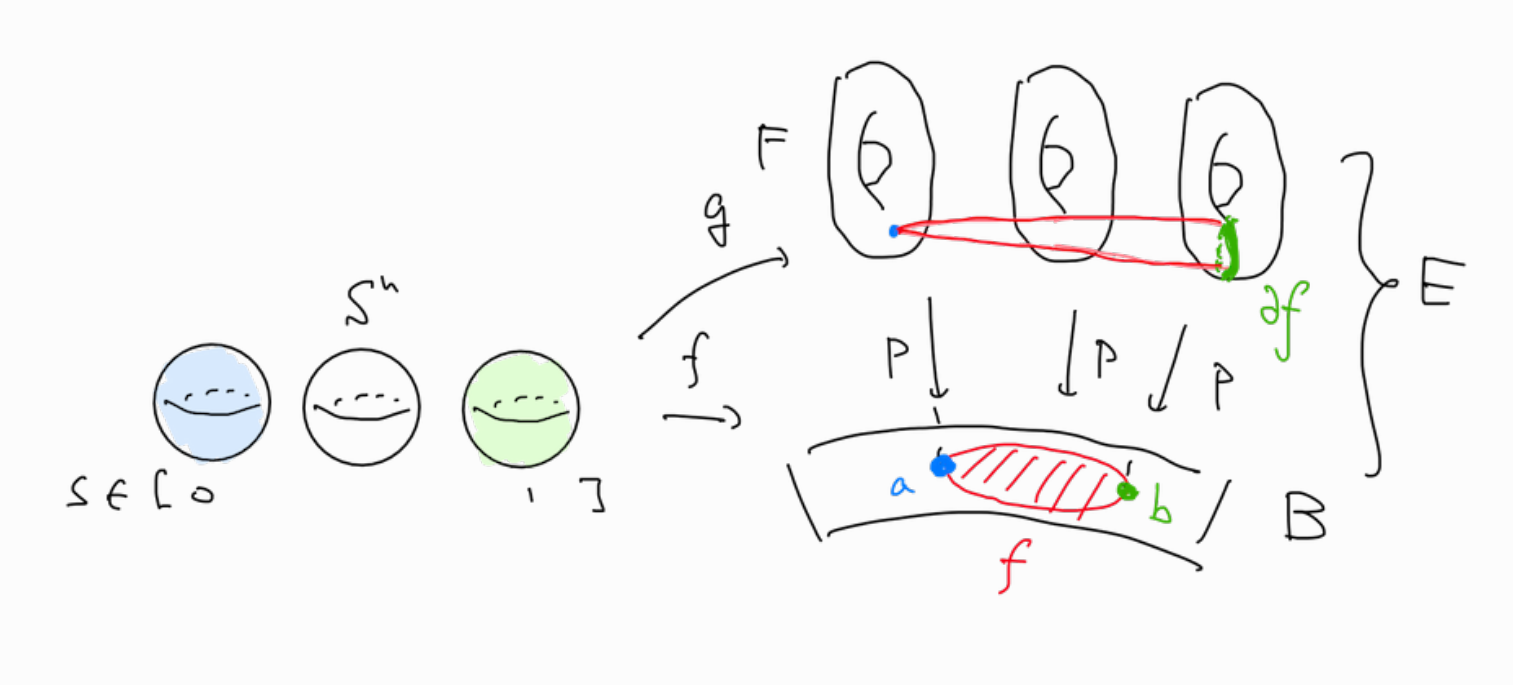
\includegraphics[width=0.72\textwidth]{figures/fig4_9.png}\\*[2pt]
{\small 图 4.9：连接映射 $\partial$}
\end{center}

定义的图示见图 4.9。

为了更好地理解连接映射，用几个例子把这个过程显式算一遍是有启发的。第一个例子，考虑纤维丛 $\Z_2\to S^1\to S^1$，其中第二个映射是 $2:1$。我们来看连接映射 $\partial$ 在下面这一段上的表现
\begin{equation}
\pi_1(\Z_2)=0\to\pi_1(S^1)=\Z\to\pi_1(S^1)=\Z\xrightarrow{\partial}\pi_0(\Z_2)=\Z_2\to\pi_0(S^1)=\Z.
\tag{4.48}
\end{equation}
为计算 $\partial$，取 $\pi_1(S^1)=\Z$ 的生成元，即恒等映射 $f:S^1\to S^1$。现在如图 4.10 所示，把源空间 $S^1$ 看成 $S^0\times[0,1]$。把它提升到全空间。如图所示，过程结束时得到恒等映射 $\tilde f(-,1):S^0\to\Z_2$，它生成 $\pi_0(\Z_2)=\Z_2$。

第二个例子，考虑与 Hopf 纤维化 $S^1\to S^3\to S^2$ 相关的下面这一段：
\begin{equation}
0=\pi_2(S^3)\to\pi_2(S^2)\xrightarrow{\partial}\pi_1(S^1)\to\pi_1(S^3)=0.
\tag{4.49}
\end{equation}
取恒等映射 $f:S^2\to S^2$，来计算 $\partial f$。对 $S^2$ 使用极坐标 $(\sin\theta\cos\phi,\sin\theta\sin\phi,\cos\theta)$。于是可以把 $\theta\in[0,\pi]$ 当作上面定义中用到的 $s\in[0,1]$，从而 $f(\phi,\theta)=(\phi,\theta)$。

% [原文 p.62]
\begin{center}
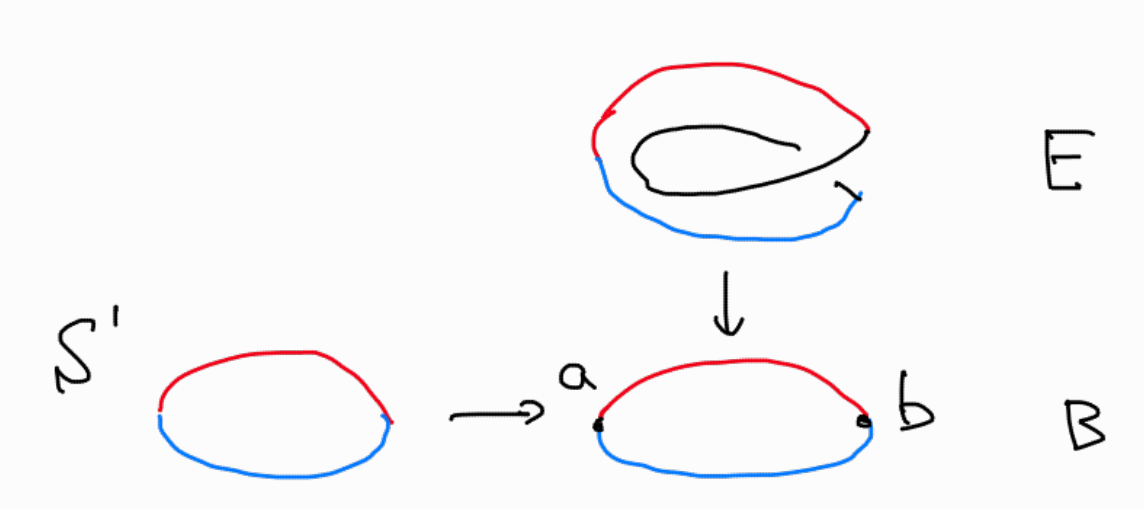
\includegraphics[width=0.66\textwidth]{figures/fig4_10.png}\\*[2pt]
{\small 图 4.10：纤维丛 $\Z_2\to S^1\to S^1$ 的连接映射 $\partial$ 图示。}
\end{center}

现在回忆 Hopf 映射 $S^3\to S^2$ 的如下描述 (3.15)：
\begin{equation}
(\cos(\theta/2)e^{i\psi},\sin(\theta/2)e^{i(\phi+\psi)})\mapsto(\sin\theta\cos\phi,\sin\theta\sin\phi,\cos\theta).
\tag{4.50}
\end{equation}
于是可以取
\begin{equation}
g(\phi,\theta):=(\cos(\theta/2),\sin(\theta/2)e^{i\phi}).
\tag{4.51}
\end{equation}
确实可以看出
\begin{equation}
(\partial f)(\phi):=g(\phi,\pi)=(0,e^{i\phi}),
\tag{4.52}
\end{equation}
它确实绕 $(0,0,1)$ 上方的纤维转了一圈。

现在对连接映射 $\partial$ 有了一些概念，就可以进入证明本身了：

\begin{proof}[证明思路]
先看这一段
\begin{equation}
\pi_n(F)\xrightarrow{\iota_*}\pi_n(E)\xrightarrow{p_*}\pi_n(B).
\tag{4.53}
\end{equation}
$p_*\circ\iota_*=0$ 是显然的。但不仅如此，我们还需要证明 $\mathrm{Im}\,\iota_*=\Ker p_*$。于是设 $f:S^n\to E$ 使得 $F=p\circ f:S^n\to B$ 同伦于平凡映射。那么就有一个形变 $F_s$（$s\in[0,1]$），使得 $F_0=F$、$F_1$ 是常值映射。在每一步 $F_s$，都能找到 $f_s:S^n\to E$ 使 $p\circ f_s=F_s$。由于 $p\circ f_0=F_0$ 是到基点的常值映射，$f_0$ 实际上是到某个纤维的映射，证毕。

接着看这一段
\begin{equation}
\pi_{n+1}(B)\xrightarrow{\partial}\pi_n(F)\xrightarrow{\iota_*}\pi_n(E).
\tag{4.54}
\end{equation}
由 $\partial$ 的定义，性质 $\mathrm{Im}\,\partial=\Ker\iota_*$ 几乎是同义反复。

最后看这一段
\begin{equation}
\pi_{n+1}(E)\xrightarrow{p_*}\pi_{n+1}(B)\xrightarrow{\partial}\pi_n(F).
\tag{4.55}
\end{equation}
同样，性质 $\mathrm{Im}\,p_*=\Ker\partial$ 几乎是同义反复。定理的证明梗概到此结束。
\end{proof}

\takeaway{纤维丛 $F\to E\to B$ 给出同伦群的长正合列，把纤维、全空间与底空间的同伦群串成一条链；知道其中两个，往往就能定出第三个。连接映射 $\partial$ 用 $S^n\times[0,1]$ 的提升显式构造，正合性因此几乎是同义反复。}

% [原文 p.63]
\section{李群的同伦群}

要使用同伦群长正合列，我们得先知道一些同伦群。前面已经给出了某些 $n,m$ 下 $\pi_n(S^m)$ 的表。这里讨论李群的同伦群。

\noindent$\pi_n(U(1))$：先从 $U(1)$ 开始。由于 $U(1)=S^1$，$\pi_n(U(1))$ 已经知道了。

\noindent$\pi_0(G)$：接着讨论非阿贝尔李群 $G$。对群而言，连通分支的集合 $\pi_0(G)$ 本身就是一个群。例如 $O(n)$ 有两个分支，一个 $\det=+1$，另一个 $\det=-1$。于是 $\pi_0(O(n))=\Z_2$。本小节余下部分只考虑连通的李群，此时 $\pi_0(G)=1$。

\noindent$\pi_1(G)$：下面考虑 $\pi_1(G)$。

\begin{qmbox}
\qmstmt{事实}{4.57}已知 $\Gamma$ 总是阿贝尔群。此外还已知，总存在群 $\tilde G$ 满足 $\pi_1(\tilde G)=0$，并配有子群 $\Gamma\subset\tilde G$，使得
\begin{equation}
G=\tilde G/\Gamma.
\tag{4.56}
\end{equation}
这样的 $\tilde G$ 称为 $G$ 的万有覆叠。
\end{qmbox}

我们来验证 $\pi_1(\tilde G/\Gamma)=\Gamma$。为此考虑纤维丛 $\Gamma\to\tilde G\to G$ 对应的同伦群长正合列，即
\begin{equation}
\pi_1(\tilde G)\to\pi_1(G)\to\pi_0(\Gamma)\to\pi_0(\tilde G).
\tag{4.57}
\end{equation}
由于 $\pi_1(\tilde G)=\pi_0(\tilde G)=0$，可见 $\pi_1(G)\simeq\pi_0(\Gamma)\simeq\Gamma$。

我们通常遇到的情形是 $G=SO(n)$，当 $n\ge 3$ 时 $\pi_1(SO(n))=\Z_2$，这在例 4.53 中已经看到。对应的万有覆叠是 Spin 群 $Spin(n)$；于是有
\begin{equation}
\Z_2\to Spin(n)\to SO(n).
\tag{4.58}
\end{equation}

\noindent$\pi_{2,3,4}(G)$：考虑紧李群 $G$，要求它连通（即 $\pi_0(G)=0$）且单连通（即 $\pi_1(G)=0$）。已知这样的群总是若干个 $\R$ 的副本与
\begin{equation}
SU(n\ge 2),\quad Spin(n\ge 6),\quad Sp(n\ge 2),\quad F_4,\quad G_2,\quad E_6,\quad E_7,\quad E_8
\tag{4.59}
\end{equation}
的乘积。其中 $Spin(3)=SU(2)$、$Spin(4)=SU(2)^2$、$Spin(5)=Sp(2)$、$Spin(6)=SU(4)$ 以及 $Sp(1)=SU(2)$ 因冗余已从清单中排除。

式 (4.59) 中的群称为紧、单、单连通的李群。

% [原文 p.64]
\begin{qmbox}
\qmstmt{事实}{4.58}对式 (4.59) 中的群 $G$，$\pi_2(G)=0$、$\pi_3(G)=\Z$。
\end{qmbox}

\begin{qmbox}
\qmstmt{事实}{4.59}对式 (4.59) 中的群 $G$，$\pi_4(G)$ 要么是 $\Z_2$（当 $G=Sp(n)$），要么是 $0$。
\end{qmbox}

\noindent$\pi_{n\ge 5}(G)$：我们在表 2 中列出单连通李群的同伦群 $\pi_n(G)$，$3\le n\le 11$。数据取自 [日07、附录、公式 7、VII]。（同一套表应当也包含在英译本 [Itö87] 中。）

\newcommand{\tBcell}[1]{\makebox[3.9em][c]{\rule[-0.3em]{0pt}{1.5em}#1}}%
\newcommand{\tBgray}[1]{\colorbox{black!8}{\makebox[3.9em][c]{\rule[-0.3em]{0pt}{1.5em}#1}}}%
\newcommand{\tBlab}[1]{\makebox[3.4em][r]{#1}}%
\begin{center}
\begin{minipage}{\linewidth}
\centering
\footnotesize
\setlength{\fboxsep}{0pt}%
\setlength{\tabcolsep}{0pt}%
\begin{tabular}{c|*{10}{c}}
\hline
\tBlab{$G\backslash d$} & \tBcell{2} & \tBcell{3} & \tBcell{4} & \tBcell{5} & \tBcell{6} & \tBcell{7} & \tBcell{8} & \tBcell{9} & \tBcell{10} & \tBcell{11}\\
\hline
\tBlab{$Sp(1)$} & \tBgray{0} & \tBcell{$\Z$} & \tBcell{$\Z_2$} & \tBcell{$\Z_2$} & \tBcell{$\Z_{12}$} & \tBcell{$\Z_2$} & \tBcell{$\Z_2$} & \tBcell{$\Z_3$} & \tBcell{$\Z_{15}$} & \tBcell{$\Z_2$}\\
\tBlab{$Sp(2)$} & \tBgray{0} & \tBcell{$\Z$} & \tBcell{$\Z_2$} & \tBcell{$\Z_2$} & \tBgray{0} & \tBcell{$\Z$} & \tBgray{0} & \tBgray{0} & \tBcell{$\Z_{120}$} & \tBcell{$\Z_2$}\\
\tBlab{$Sp(3)$} & \tBgray{0} & \tBcell{$\Z$} & \tBcell{$\Z_2$} & \tBcell{$\Z_2$} & \tBgray{0} & \tBcell{$\Z$} & \tBgray{0} & \tBgray{0} & \tBgray{0} & \tBcell{$\Z$}\\
\hline
\tBlab{$SU(3)$} & \tBgray{0} & \tBcell{$\Z$} & \tBgray{0} & \tBcell{$\Z$} & \tBcell{$\Z_6$} & \tBgray{0} & \tBcell{$\Z_{12}$} & \tBcell{$\Z_3$} & \tBcell{$\Z_{30}$} & \tBcell{$\Z_4$}\\
\tBlab{$SU(4)$} & \tBgray{0} & \tBcell{$\Z$} & \tBgray{0} & \tBcell{$\Z$} & \tBgray{0} & \tBcell{$\Z$} & \tBcell{$\Z_{24}$} & \tBcell{$\Z_2$} & \tBcell{$\Z_{120}\times\Z_2$} & \tBcell{$\Z_4$}\\
\tBlab{$SU(5)$} & \tBgray{0} & \tBcell{$\Z$} & \tBgray{0} & \tBcell{$\Z$} & \tBgray{0} & \tBcell{$\Z$} & \tBgray{0} & \tBcell{$\Z$} & \tBcell{$\Z_{120}$} & \tBgray{0}\\
\tBlab{$SU(6)$} & \tBgray{0} & \tBcell{$\Z$} & \tBgray{0} & \tBcell{$\Z$} & \tBgray{0} & \tBcell{$\Z$} & \tBgray{0} & \tBcell{$\Z$} & \tBgray{0} & \tBcell{$\Z$}\\
\hline
\tBlab{$Spin(7)$} & \tBgray{0} & \tBcell{$\Z$} & \tBgray{0} & \tBgray{0} & \tBgray{0} & \tBcell{$\Z$} & \tBcell{$(\Z_2)^2$} & \tBcell{$(\Z_2)^2$} & \tBcell{$\Z_8$} & \tBcell{$\Z\times\Z_2$}\\
\tBlab{$Spin(8)$} & \tBgray{0} & \tBcell{$\Z$} & \tBgray{0} & \tBgray{0} & \tBgray{0} & \tBcell{$\Z^2$} & \tBcell{$(\Z_2)^3$} & \tBcell{$(\Z_2)^3$} & \tBcell{$\Z_{24}\times\Z_8$} & \tBcell{$\Z\times\Z_2$}\\
\tBlab{$Spin(9)$} & \tBgray{0} & \tBcell{$\Z$} & \tBgray{0} & \tBgray{0} & \tBgray{0} & \tBcell{$\Z$} & \tBcell{$(\Z_2)^2$} & \tBcell{$(\Z_2)^2$} & \tBcell{$\Z_8$} & \tBcell{$\Z\times\Z_2$}\\
\tBlab{$Spin(10)$} & \tBgray{0} & \tBcell{$\Z$} & \tBgray{0} & \tBgray{0} & \tBgray{0} & \tBcell{$\Z$} & \tBcell{$\Z_2$} & \tBcell{$\Z\times\Z_2$} & \tBcell{$\Z_4$} & \tBcell{$\Z$}\\
\tBlab{$Spin(11)$} & \tBgray{0} & \tBcell{$\Z$} & \tBgray{0} & \tBgray{0} & \tBgray{0} & \tBcell{$\Z$} & \tBcell{$\Z_2$} & \tBcell{$\Z_2$} & \tBcell{$\Z_2$} & \tBcell{$\Z$}\\
\tBlab{$Spin(12)$} & \tBgray{0} & \tBcell{$\Z$} & \tBgray{0} & \tBgray{0} & \tBgray{0} & \tBcell{$\Z$} & \tBcell{$\Z_2$} & \tBcell{$\Z_2$} & \tBgray{0} & \tBcell{$\Z\times\Z$}\\
\tBlab{$Spin(13)$} & \tBgray{0} & \tBcell{$\Z$} & \tBgray{0} & \tBgray{0} & \tBgray{0} & \tBcell{$\Z$} & \tBcell{$\Z_2$} & \tBcell{$\Z_2$} & \tBgray{0} & \tBcell{$\Z$}\\
\hline
\tBlab{$G_2$} & \tBgray{0} & \tBcell{$\Z$} & \tBgray{0} & \tBgray{0} & \tBcell{$\Z_3$} & \tBgray{0} & \tBcell{$\Z_2$} & \tBcell{$\Z_6$} & \tBgray{0} & \tBcell{$\Z\times\Z_2$}\\
\tBlab{$F_4$} & \tBgray{0} & \tBcell{$\Z$} & \tBgray{0} & \tBgray{0} & \tBgray{0} & \tBgray{0} & \tBcell{$\Z_2$} & \tBcell{$\Z_2$} & \tBgray{0} & \tBcell{$\Z\times\Z_2$}\\
\tBlab{$E_6$} & \tBgray{0} & \tBcell{$\Z$} & \tBgray{0} & \tBgray{0} & \tBgray{0} & \tBgray{0} & \tBgray{0} & \tBcell{$\Z$} & \tBgray{0} & \tBcell{$\Z$}\\
\tBlab{$E_7$} & \tBgray{0} & \tBcell{$\Z$} & \tBgray{0} & \tBgray{0} & \tBgray{0} & \tBgray{0} & \tBgray{0} & \tBgray{0} & \tBgray{0} & \tBcell{$\Z$}\\
\tBlab{$E_8$} & \tBgray{0} & \tBcell{$\Z$} & \tBgray{0} & \tBgray{0} & \tBgray{0} & \tBgray{0} & \tBgray{0} & \tBgray{0} & \tBgray{0} & \tBgray{0}\\
\hline
\end{tabular}\\[3pt]
{\small 表 2：单连通单李群的同伦群 $\pi_d(G)$，$2\le d\le 11$。}
\end{minipage}
\end{center}

我们注意到，把同伦群长正合列用到
\begin{equation}
\begin{array}{cccccc}
Spin(n-1) & \to & Spin(n) & \to & S^{n-1}, &\\
SU(n-1) & \to & SU(n) & \to & S^{2n-1}, &\\
Sp(n-1) & \to & Sp(n) & \to & S^{4n-1} &
\end{array}
\tag{4.60}
\end{equation}

% [原文 p.65]
就得到
\begin{equation}
\pi_d(Spin(n-1))\simeq\pi_d(Spin(n)),
\tag{4.61}
\end{equation}
\begin{equation}
\pi_d(SU(n-1))\simeq\pi_d(SU(n)),
\tag{4.62}
\end{equation}
\begin{equation}
\pi_d(Sp(n-1))\simeq\pi_d(Sp(n))
\tag{4.63}
\end{equation}
分别当 $d<n-2$、$d<2n-2$、$d<4n-2$ 时成立。这与表 2 的数据一致，也使我们能一致地定义 $\pi_d(Spin(\infty))$、$\pi_d(SU(\infty))$ 与 $\pi_d(Sp(\infty))$。

\takeaway{李群的低阶同伦群容易描述：$\pi_0$ 数连通分支，$\pi_1$ 由万有覆叠给出，如 $\Z_2\to Spin(n)\to SO(n)$；$\pi_2=0$、$\pi_3=\Z$，$\pi_4$ 除 $Sp(n)$ 为 $\Z_2$ 外皆 $0$。单连通单李群的 $\pi_d$（$2\le d\le 11$）见表 2，其数值由三条李群丛的长正合列给出。}

\section{球面上的主丛}

下面用同伦群来分类球面上的主丛。

\subsection{一般性}

从一般构造开始。

\begin{definition}{4.60}
给定丛 $F\to E\xrightarrow{p}B$ 与映射 $f:X\to B$，拉回丛 $p':f^*(E)\to X$ 定义为
\begin{equation}
f^*(E)=\{(x,e)\in X\times E\mid f(x)=p(e)\},
\tag{4.64}
\end{equation}
其中 $p'((x,e))=x$。
\end{definition}

可以用 $E$ 的局部平凡化显式给出 $f^*(E)$ 的局部平凡化。设有 $B$ 的开集覆盖 $U_i$ 以及 $E$ 的局部平凡化 $f_i:p^{-1}(U_i)\to U_i\times F$。记 $f_i(e)=(p(e),F_i(e))$。用 $V_i:=f^{-1}(U_i)$ 覆盖 $X$，并通过把
\begin{equation}
(x,e)\in p'^{-1}(V_i)
\tag{4.65}
\end{equation}
映到
\begin{equation}
(x,F_i(e))\in V_i\times F
\tag{4.66}
\end{equation}
来定义局部平凡化。

\begin{theorem}{4.61}
给定丛 $F\to E\to B$ 与两个彼此同伦的映射 $f,g:X\to B$，拉回丛 $f^*(E)$ 与 $g^*(E)$ 作为丛是等价的。
\end{theorem}

回忆一下，丛的等价在定义 3.3 中已经定义。这个重要定理的证明值得一看，但可惜我们没有时间。

\begin{proposition}{4.62}
设 $U$ 是可缩空间。则 $U$ 上的任何丛都是平凡的。
\end{proposition}

这容易由前一定理推出。事实上，取一点 $p\in U$。则恒等映射 $\id:U\to U$ 同伦于把所有点都送到 $p$ 的常值映射 $f:U\to U$。因此 $E=\id^*(E)$ 等价于 $f^*(E)=U\times F$，而后者是平凡的。

% [原文 p.66]
现在考虑主 $G$-丛 $G\to P\to S^n$。用北半球与南半球 $U_+$、$U_-$ 覆盖 $S^n$，并让两块区域在赤道附近略有重叠。可以在每个半球上把丛平凡化，于是丛 $P$ 由 $U_+\times G$ 与 $U_-\times G$ 在重叠部分借助函数 $g:U_+\cap U_-\to G$ 粘合而成。由于 $U_+\cap U_-$ 可缩到赤道 $S^{n-1}$，丛由映射 $S^{n-1}\to G$ 决定。而同伦的映射决定等价的丛，于是得到

\begin{proposition}{4.63}
球面 $S^n$ 上的主 $G$-丛由 $\pi_{n-1}(G)$ 分类。
\end{proposition}

\subsection{例}

有两个标准例子。先从 $S^2$ 上的 $U(1)$ 丛开始。它由 $\pi_1(U(1))=\pi_1(S^1)=\Z$ 分类。

在物理中，要研究拓扑非平凡情形下的电磁学，就需要 $U(1)$ 丛。后面会知道，这个整数就是磁荷，等价地，就是穿过 $S^2$ 的磁单极子磁通量。为此需要引入联络的概念，等价地，就是规范场。这将给出这个数的微分几何表达式，即磁场在 $S^2$ 上的积分。

磁荷是量子化的，这一点最早由 Dirac [Dir31] 发现。\footnote[12]{有趣的是，这项工作与 Hopf 引入 Hopf 不变量和 Hopf 纤维化 $S^1\to S^3\to S^2$ 是在同一年 [Hop31]，后者同样关于 $S^2$ 上非平凡的 $U(1)$ 丛。}这里用的是几何论证，因此磁荷的单位是无量纲的，并被取为 $1$。后面我们会看到如何把这个单位与你喜欢的电磁学单位制联系起来。总结如下：

\begin{example}{4.64}
$S^2$ 上的 $U(1)$ 丛由 $\pi_1(U(1))=\Z$ 分类。这在物理中对应磁通量。
\end{example}

接着考虑 $S^3$ 上的 $G$-丛，其中 $G$ 是单、单连通的紧李群，例如 $SU(2)$。对这类群，$\pi_3(G)=\Z$，这是上面学到的。

在物理中，更常见的是考虑平坦 $\R^4$ 上的主丛 $P\to\R^4$，我们把 $\R^4$ 当作我们世界的良好近似。进一步假设在无穷远处有平凡化：若挖掉一个发生有趣事情的有限区域 $U\subset\R^4$，在时空的其余部分 $U'=\R^4\setminus U$ 上什么也没发生，并且那里给定了局部平凡化 $U'\times G$。于是可以有效地把区域 $U'$ 看作一个点，并把我们的丛看成某个主 $G$-丛 $P\to S^4$ 的拉回，见图 4.11。这样 $G$-丛的拓扑由一个整数 $\pi_3(G)=\Z$ 刻画。这个数在物理中称为瞬子数。后面我们还会给出这个数的微分几何解释。

注意，丛在无穷远处平凡这个假设来自物理，并非数学上的必然。若对无穷远处作其他假设，对应不同的物理设定，就会得到其他分类。还要提到，$T^4$ 上丛的分类要困难得多。

% [原文 p.67]
\begin{center}
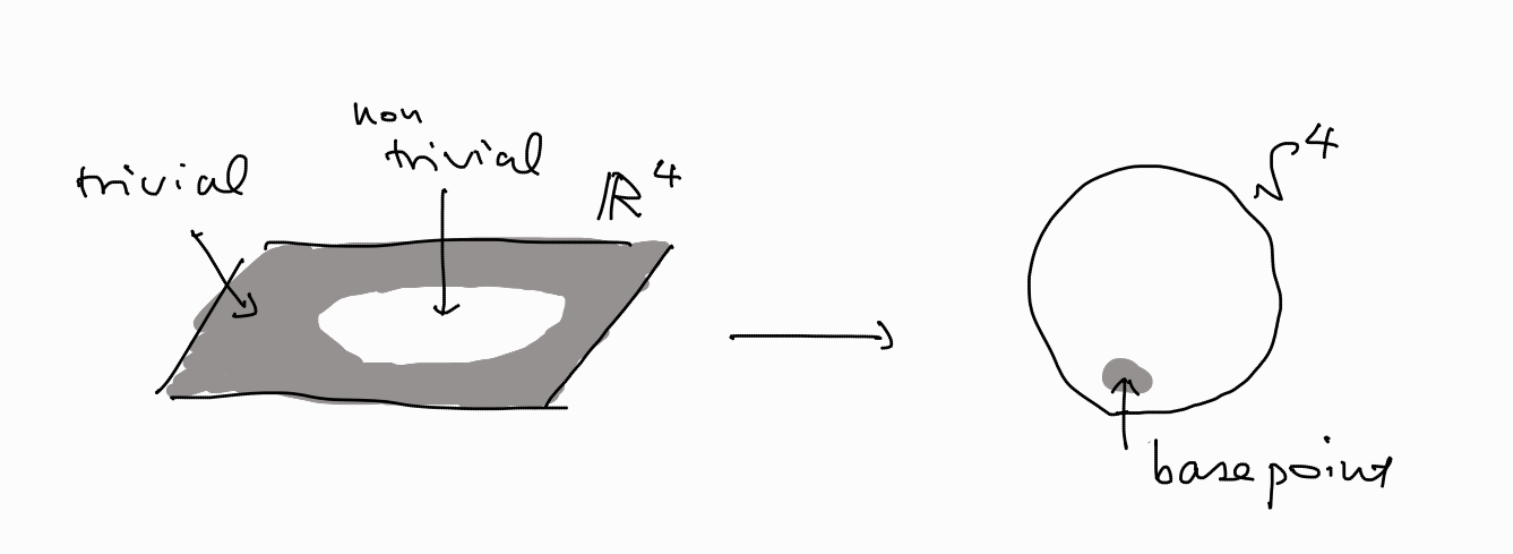
\includegraphics[width=0.78\textwidth]{figures/fig4_11.png}\\*[2pt]
{\small 图 4.11：$\R^4$ 上在无穷远处平凡化的主丛由 $S^4$ 的拉回给出。}
\end{center}

无论如何，总结一下：

\begin{example}{4.65}
对单、单连通的紧李群 $G$（例如 $SU(2)$），$S^4$ 上的主 $G$-丛由 $\pi_3(G)=\Z$ 分类。这在物理中称为瞬子数。
\end{example}

\subsection{重访同伦群的长正合列}

本小节的结果可以让我们换一个角度看同伦群的长正合列。

先讨论连接同态 $\partial$。回忆我们有主 $H$-丛 $H\to G\to G/H$。取一个类 $[f]\in\pi_n(G/H)$。这样就有了映射 $f:S^n\to G/H$。可以用它把 $H$-丛 $G\to G/H$ 拉回到 $S^n$，得到主 $H$-丛 $f^*(G)\to S^n$。根据球面上主丛的分类，它应当由 $\pi_{n-1}(H)$ 中的一个类来分类。这样就构造了映射 $\pi_n(G/H)\to\pi_{n-1}(H)$。要说明它等于定义 4.56 中给出的连接同态 $\partial$，基本上只是把涉及的各种定义展开一遍，没有别的内容。总结起来，我们得到：

\begin{proposition}{4.66}
给定映射 $f:S^n\to G/H$，把 $G\to G/H$ 拉回得到的主 $H$-丛 $f^*(G)\to S^n$ 由类 $\partial[f]\in\pi_{n-1}(H)$ 分类。
\end{proposition}

\takeaway{球面 $S^n$ 上的主 $G$-丛由 $\pi_{n-1}(G)$ 分类：$S^2$ 上的 $U(1)$ 丛给出磁通量，$S^4$ 上的丛给出瞬子数。拉回丛在底空间的同伦下不变，而长正合列中的连接同态正是这种分类的体现。}

\section{拓扑孤子与同伦群}

现在来到代数拓扑在物理中最传统的应用，即拓扑孤子的研究。

% [原文 p.68]
\subsection{无芯孤子，又称织构（textures）}

假设我们的空间（时空）上有一个场，取值于目标空间 $X$，也就是说有一个映射
\begin{equation}
f:\R^D\to X. \tag{4.67}
\end{equation}
我们常考虑沿某些方向具有（近似）平移不变性的情形。这时场组态的非平凡性由一个映射
\begin{equation}
f:\R^d\to X \tag{4.68}
\end{equation}
刻画。

这时场组态沿 $d'=D-d$ 个方向为常量。我们称 $d$ 为该组态的余维数。见图 4.12。这时讨论它在 $d'$ 方向上单位体积的能量（或张力）是有意义的。为简单起见，取 $d'=0$；这在此处的分析中没有区别，于是我们干脆把单位体积的能量称为能量。

\begin{center}
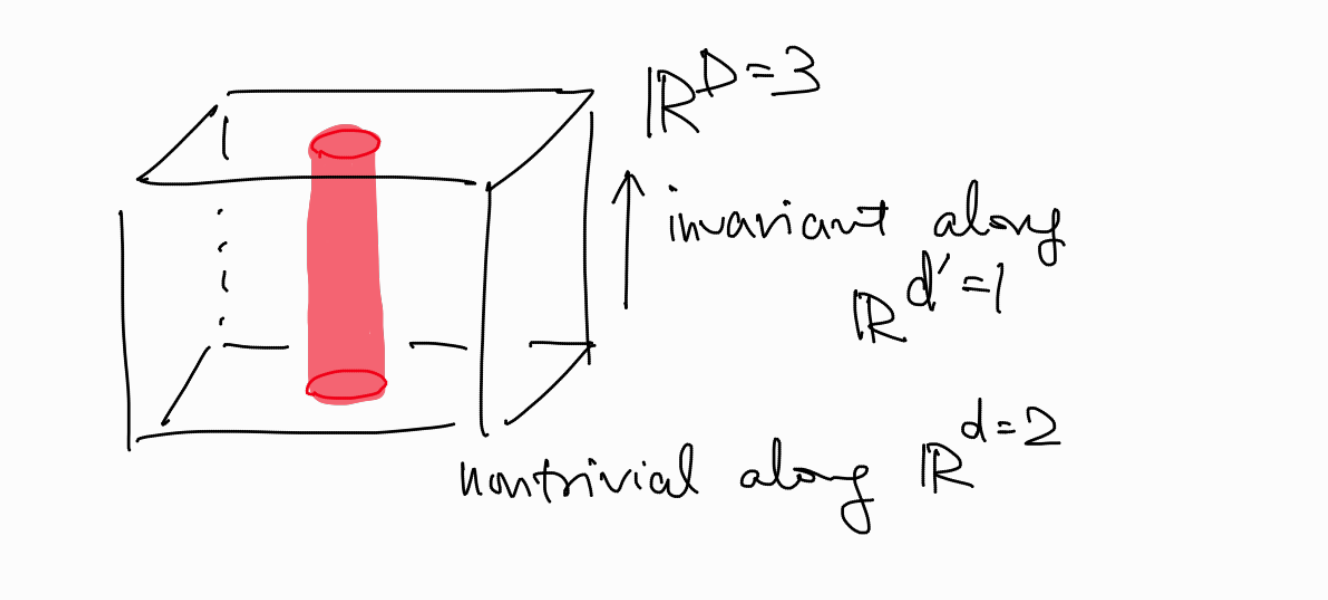
\includegraphics[width=0.72\textwidth]{figures/fig4_12.png}\\*[2pt]
{\small 图 4.12：$\R^3$ 中余维 2 的物体呈弦状。}
\end{center}

现在，为了不在渐近远处花费无穷多的能量，$\R^d$ 的大部分区域必须映射到目标空间 $X$ 中某个点的近旁。我们把这个点取作 $X$ 的基点，于是这样的映射本质上由从 $S^d$ 出发的映射给出。见图 4.13。

这样的组态于是决定一个同伦类 $[f]\in\pi_d(X)$。若 $[f]$ 非零，它就无法通过连续过程消除，因此给出一个拓扑守恒荷；带有这种拓扑守恒荷的组态称为拓扑孤子。

\begin{example}{4.67}
取余维数 $3$、目标空间 $S^3$，就得到 Skyrmion，其荷由 $\pi_3(S^3)=\Z$ 给出。
\end{example}

这最早由 Skyrme\footnote[13]{在日本，Skyrmion 一词有时读作 [skirmion]，但我认为 [skə:miən] 更正确；毕竟 T. H. R. Skyrme 是英国人，而我认为 [skirmion] 是一种矫枉过正。至于 Ising 模型，我认为应当用 [i:ziŋ] 而不是 [aiziŋ]，因为 E. Ising 是德国人。说到本领域常见人名的发音，Källen--Lehmann 谱表示中 Källen 的发音也很麻烦。我常听到比我年长的高能物理学家把它读成 [chælən] 之类。Källen 是瑞典人，Källen 的孙辈在做弦论，我见过他几次。他告诉我正确的发音，在我听来接近 [shælien]，与维基百科上关于标准瑞典语发音的页面相差很大。} [Sky61, Sky62] 在把核子看作介子场中的孤子的背景下引入。

% [原文 p.69]
\begin{center}
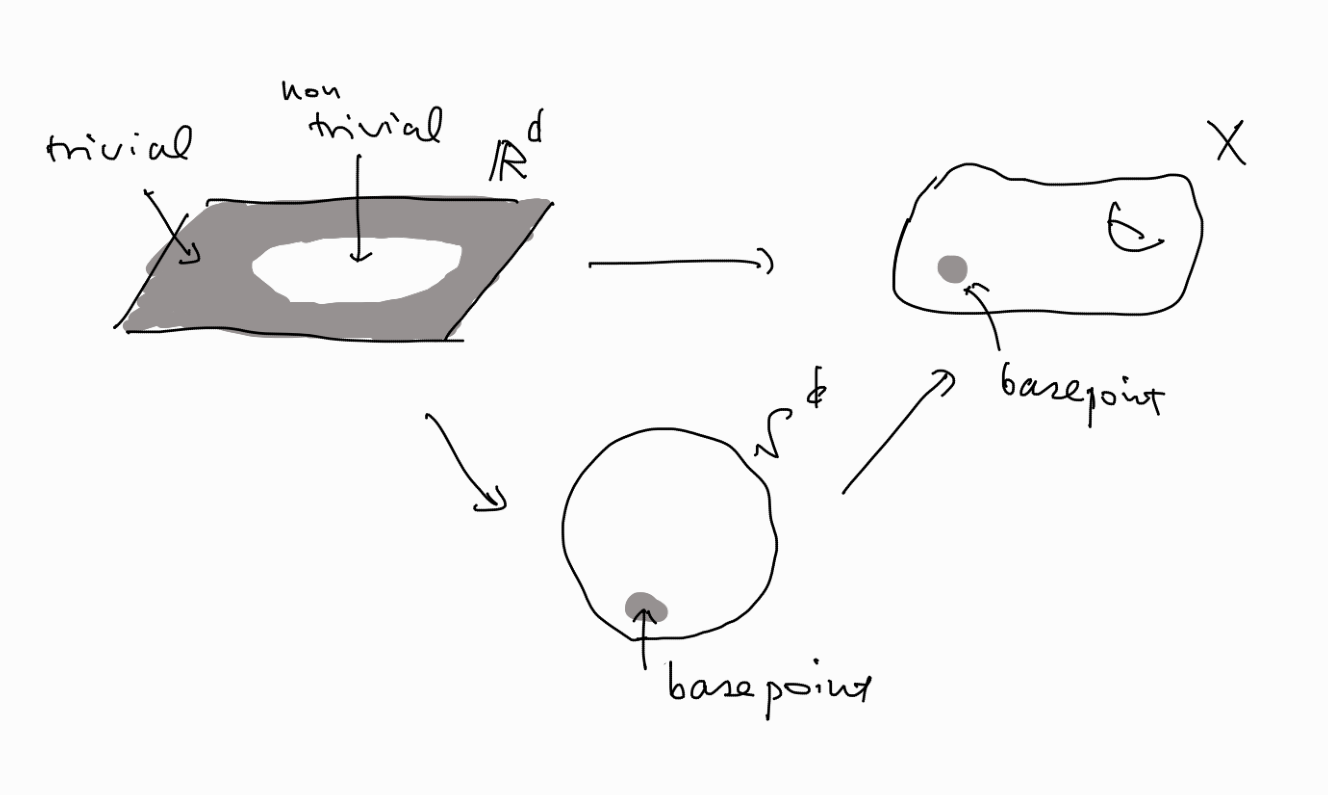
\includegraphics[width=0.66\textwidth]{figures/fig4_13.png}\\*[2pt]
{\small 图 4.13：光滑、有限能量、余维 $d$ 的组态由映射 $S^d\to X$ 给出。}
\end{center}

\begin{example}{4.68}
取余维数 $2$、目标空间 $S^2$，就得到 baby Skyrmion，其荷由 $\pi_2(S^2)=\Z$ 给出。baby Skyrmion 常简称为 Skyrmion。
\end{example}

快速上网搜索一下，就能找到大量 Skyrmion 的实验实现，但其中大多数似乎是 baby Skyrmion。

\begin{example}{4.69}
取余维数 $3$、目标空间 $S^2$，就得到 Hopfion，其荷由 $\pi_3(S^2)=\Z$ 给出。
\end{example}

再快速上网搜一下，也能找到一些 Hopfion 的实验实现。另一个值得注意之处是，Hopfion 的荷比 Skyrmion 的荷更微妙；如果你感兴趣，可以查阅一篇最近的论文 [CT22]，\footnote[14]{我提到这一点，是因为我曾自豪地担任这篇论文年轻作者的博士答辩委员会主席。}该文指出 Hopfion 的荷与一种非可逆对称性相关，这是近年来的热门话题。

\subsection{有芯孤子，更常称为拓扑缺陷}

\para{一般性：}下面看看可以称为有芯孤子的东西。考虑余维 $d$ 的组态，它带有到目标空间 $X$ 的映射，其中

% [原文 p.70]
$X$ 是序参量的空间。这里考虑图 4.14 所示的情形：映射定义在核心区域 $U\subset\R^d$ 之外。因此有一个映射
\begin{equation}
f:\R^d\setminus U\to X. \tag{4.69}
\end{equation}

\begin{center}
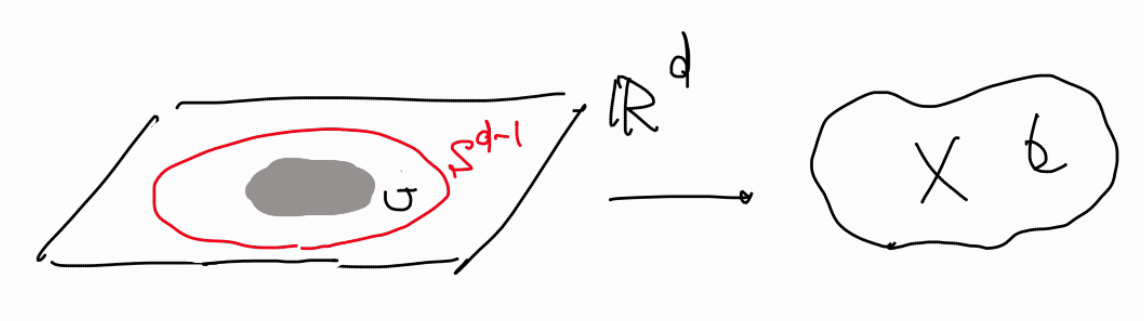
\includegraphics[width=0.72\textwidth]{figures/fig4_14.png}\\*[2pt]
{\small 图 4.14：带“核心”的余维 $d$ 组态，由映射 $S^{d-1}\to X$ 给出。}
\end{center}

这时，这种映射的非平凡性由映射 $f:S^{d-1}\to X$ 的同伦类 $[f]\in\pi_{d-1}(X)$ 衡量。注意它与上面讨论的光滑余维 $d$ 孤子用 $\pi_d(X)$ 衡量的拓扑荷的区别。

注意，若 $[f]$ 非平凡，它就绝不可能光滑地延拓到整个 $U$ 上。因为若可以，所得映射 $D^d\to X$ 就给出同伦，表明 $[f]$ 平凡。

当 $[f]$ 非平凡时，我们就无法把映射 $f$ 连续延拓到整个 $U$ 上。在区域 $U$ 内部，我们假设发生了某种超出“仅有一个以 $X$ 为参数的序参量场”的额外物理。这在物理中很容易发生：通常空间 $X$ 只作为低能近似出现。这时正是在区域 $U$ 中，低能近似失效了。

还要注意，若 $[f]$ 非平凡，$f$ 的位置依赖通常在渐近远处要花费无穷多的能量。但在一些物理情形中，这个问题可能无关紧要：

\begin{itemize}
\item 其一，实验装置是有限的，因此无限大 $\R^d$ 中的无穷能量可能无关紧要；
\item 其二，当 $X=G/H$ 且 $G$ 与规范场相关时，渐近远处一个非平凡的 $G$-规范变换可以去掉这种位置依赖，从而去掉相应的无穷多能量。
\end{itemize}

因此本讲中我们忽略这些能量方面的考虑。

\para{涡旋：}说明上述讨论的一个例子是 $X=S^1$。序参量空间 $S^1$ 作为酒瓶势的势能极小值空间出现，这已在 §2.4.3 中看到。这时可以考虑图 4.15 所示的场组态。在渐近远处，我们让场值随着绕核心一圈而绕势能极小值 $S^1$ 一周。在核心区域，场空间 $\R^2$ 中的这个 $S^1$ 需要收缩。这与额外的势能相关，但它被限制在空间中一个有限的核心区域内，因此

% [原文 p.71]
\begin{center}
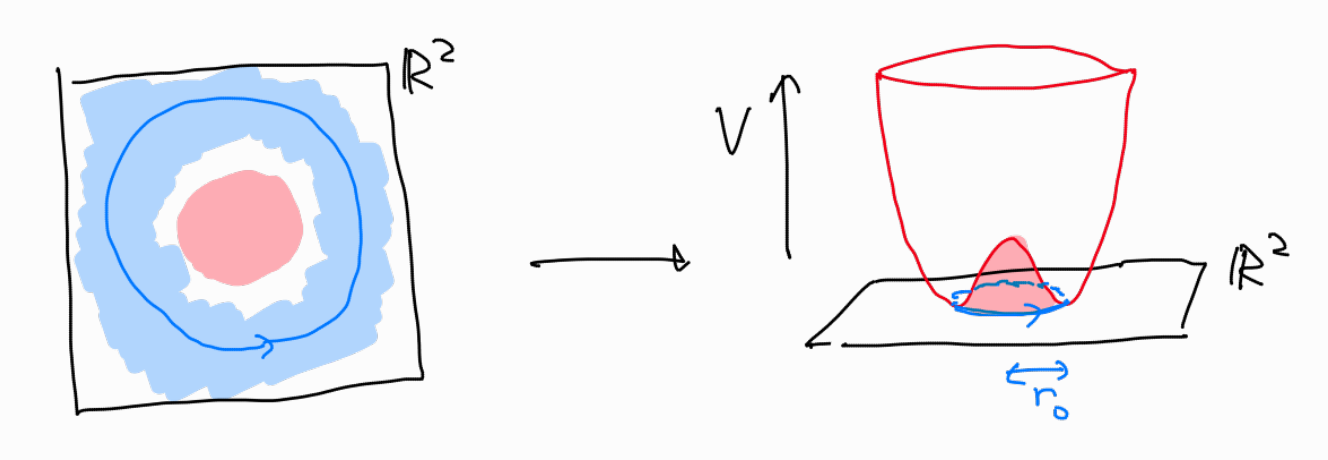
\includegraphics[width=0.62\textwidth]{figures/fig4_15.png}\\*[2pt]
{\small 图 4.15：涡旋组态。渐近区域场值位于势能底部，核心区域场值来到场空间的原点。}
\end{center}

这样只花费有限的能量。注意在远处，对称性从 $G=U(1)=S^1$ 破缺到平凡群 $H=\{e\}$；但在核心区域的至少一个点上，整个对称性 $G=U(1)$ 都未破缺。于是，在拓扑孤子的核心，对称性被迫恢复。

这种涡旋组态最早由 Abrikosov [Abr57] 在凝聚态物理的超导背景下引入，并由 Nielsen 与 Olesen [NO73] 在高能物理中引入。如今这些涡旋已在实验上被观测到，见图 4.16。总结起来：

\begin{center}
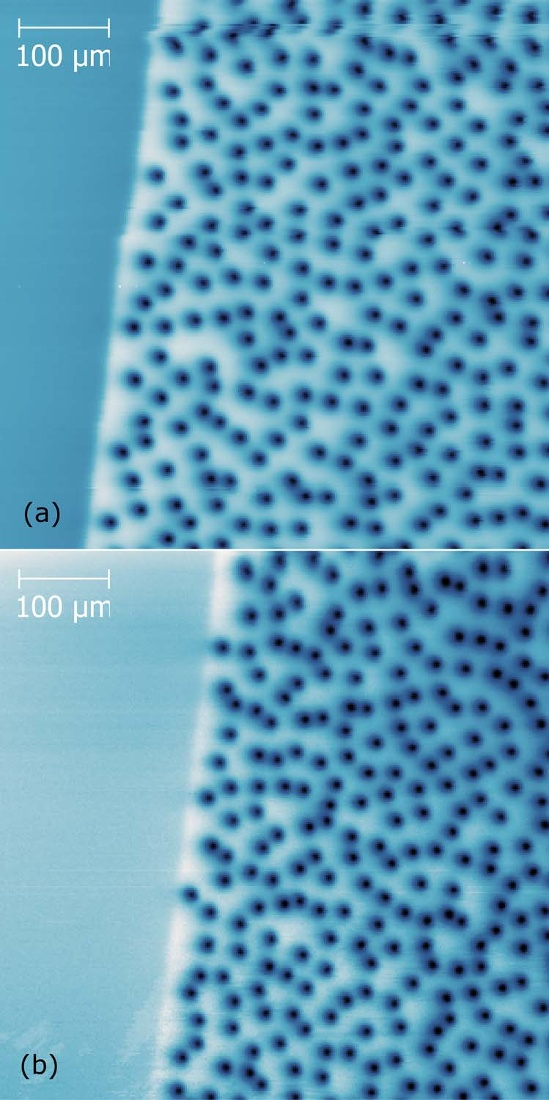
\includegraphics[width=0.30\textwidth]{figures/fig4_16.png}\\*[2pt]
{\scriptsize \textbf{Figure 1} $\mid$ Images of vortices in 200 nm thick YBCO film taken by Scanning SQUID Microscopy after field cooling at 6.93 $\mu$T to 4 K. (b) is taken after heating above $T_c$ and re-cooling. The sample edge at the left side of the images is used as a reference for scan location.}\\*[1pt]
{\small 图 4.16：超导材料中涡旋的扫描 SQUID 显微图像。取自 [WPW+15]。}
\end{center}

% [原文 p.72]
\begin{example}{4.70}
余维数为 $2$ 的带芯拓扑孤子，若其参数空间为 $X=U(1)$，并由 $\pi_1(U(1))=\Z$ 刻画，就称为 Abrikosov--Nielsen--Olesen 涡旋。
\end{example}

\noindent\textbf{附注 4.71.}同样思路的另一个应用，是给出代数基本定理的一个证明。考虑复系数 $n$ 次多项式
\begin{equation}
P(z)=z^n+c_1z^{n-1}+\cdots+c_n.
\tag{4.70}
\end{equation}
假设 $P(z)$ 没有零点。于是总可以无歧义地写成 $P(z)=|P(z)|e^{i\theta(z)}$，从而定义一个映射
\begin{equation}
\theta:\C\to S^1.
\tag{4.71}
\end{equation}
把 $\theta$ 限制到 $\C$ 中半径 $r$ 的圆 $z=re^{i\varphi}$ 上。当 $r$ 很小时，$P(z)\sim c_n$，缠绕数显然为零；当 $r$ 很大时，$P(z)\sim z^n$，缠绕数为 $n$。由于 $r$ 连续变化时缠绕数应保持不变，这不可能发生。因此 $P(z)$ 至少有一个零点，设为 $z=z_0$。于是 $P(z)=(z-z_0)Q(z)$。

如果你更喜欢物理类比，就说 $P(z)$ 给出一个场组态。于是在核心之外有到 $S^1$ 的映射。$r$ 大时缠绕数为 $n$。因此至少应当有一个核心，在那里 $P(z)$ 为零。\qedmark

回到代数拓扑的物理解释，我们进一步把这里的 $G=U(1)$ 等同于电磁 $U(1)$。这时可以证明核心区域含有单位磁通量，做法如下；后面我们还会给出用向量势的更传统做法。为了从拓扑上测量磁通量，试着把这个组态放到 $S^2$ 上，并利用 §4.6 的结果。先把组态放在一个大的 $D^2$ 上，把它看作北半球。赤道 $L$ 附近有一个区域 $B$，那里有乘积丛 $B\times S^1$。为了一般性，设绕赤道一周时场值绕 $S^1$ 转 $N$ 圈。

再引入另一个 $D^2$，作为南半球。在它上面取平凡丛 $D^2\times S^1$ 和一个常值截面。为了把两个半球粘起来并使截面吻合，需要用 $U(1)$ 规范变换 $g:S^1\to S^1$，它同样绕 $S^1$ 转 $N$ 圈。这意味着在所得的 $S^2$ 上，$U(1)$ 丛由 $N\in\pi_1(S^1)\simeq\Z$ 刻画，因而带有磁荷 $N$。图示见图 4.17。

\para{瞬子粒子：}虽然与大自然没有直接关系，但至少在数学层面，我们可以把 $\pi_1(U(1))=\Z$ 换成 $\pi_3(SU(2))$，并考虑 $(4+1)$ 维系统中的一个余维 $4$ 粒子：

\begin{example}{4.72}
可以考虑参数空间为 $X=SU(2)$ 的余维 $4$ 带芯拓扑孤子。
\end{example}

例如，一叠 D4-膜中的一根 D0-膜就有这样的实现；这里 D$p$-膜是弦论中的 $(p+1)$ 维孤子物体。

注意 §4.6.3 中的论证表明，这个孤子的核心带有瞬子荷 $1$，同样由 $\pi_3(SU(2))=\Z$ 刻画。因此弦论中常称它为“瞬子粒子”。

% [原文 p.73]
\begin{center}
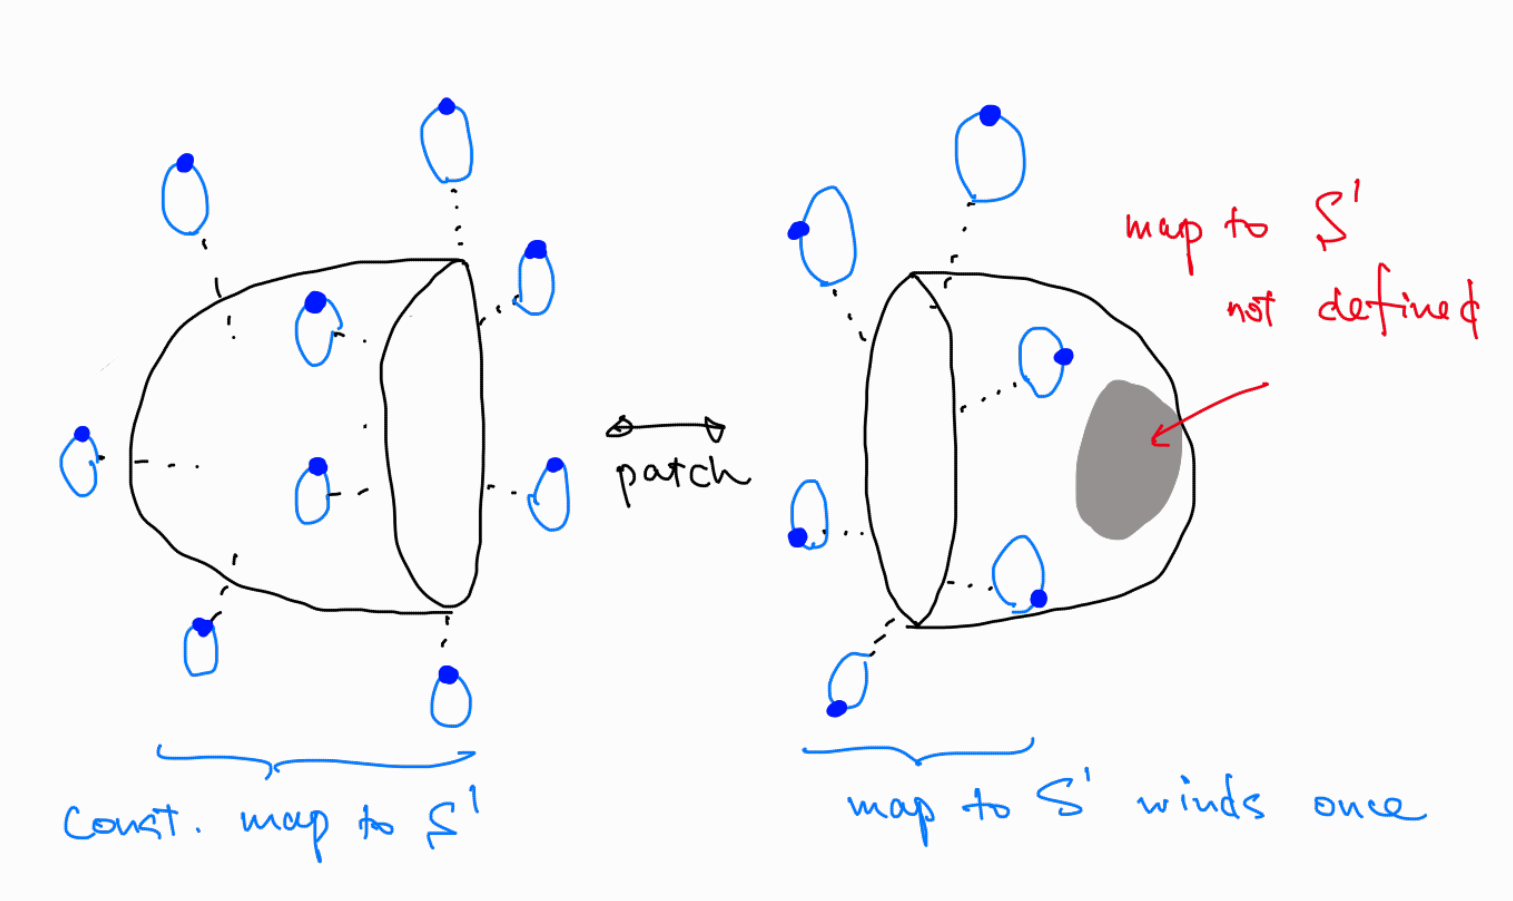
\includegraphics[width=0.62\textwidth]{figures/fig4_17.png}\\*[2pt]
{\small 图 4.17：为测量磁通量，可以把涡旋组态放到 $S^2$ 上。这需要在赤道附近有非平凡的规范变换。}
\end{center}

\para{磁单极子：}最后一个例子如下：

\begin{example}{4.73}
参数空间为 $X=S^2$ 的余维 $3$ 带芯拓扑孤子，称为 't Hooft--Polyakov 磁单极子。
\end{example}

这最早由 't Hooft [tH74] 与 Polyakov [Pol74] 引入。若把 $S^2$ 看作 $SU(2)/U(1)$，考虑一个规范理论设定：较大的群 $SU(2)$ 破缺到 $U(1)$，并把 $U(1)$ 认同为电磁规范群；则它在 $S^2$ 上带有磁荷，该荷由命题 4.66 通过同伦群长正合列中 $\pi_2(SU(2)/U(1))\to\pi_1(U(1))$ 的像来刻画，这个长正合列对应于丛 $U(1)\to SU(2)\to SU(2)/U(1)$：
\begin{equation}
\pi_2(SU(2)/U(1))\to\pi_1(U(1))\to\pi_1(SU(2))\to\pi_1(SU(2)/U(1))
\tag{4.72}
\end{equation}
即
\begin{equation}
\Z\to\Z\to 0\to 0.
\tag{4.73}
\end{equation}
正合性迫使第一个映射为恒等映射。因此，由 $1\in\pi_2(S^2)=\Z$ 刻画的最小 't Hooft--Polyakov 磁单极子带有单位磁荷 $1\in\pi_1(U(1))$。

相反，若把 $S^2$ 看作 $SO(3)/SO(2)$，并把 $SO(2)$ 认同为电磁规范群，则同样可以通过研究
\begin{equation}
\pi_2(SU(2)/U(1))\to\pi_1(SO(2))\to\pi_1(SO(3))\to\pi_1(SU(2)/U(1))
\tag{4.74}
\end{equation}
来刻画磁荷，即
\begin{equation}
\Z\to\Z\to\Z_2\to 0.
\tag{4.75}
\end{equation}

\takeaway{拓扑孤子的荷由场在无穷远处的边界条件决定：余维 $d$ 的带芯组态给出 $\pi_{d-1}(X)$，无芯组态给出 $\pi_d(X)$；涡旋、瞬子粒子与磁单极子分别对应 $\pi_1$、$\pi_3$、$\pi_2$。}

\chapterreview{本章引入代数拓扑的基本工具：同伦、同伦群与同伦等价。我们说明 $\pi_n(X)$ 对 $n\ge1$ 是群、$n\ge2$ 时是阿贝尔群，并算出球面的同伦群：$\pi_n(S^m)=0$（$n<m$）、$\pi_n(S^n)=\Z$，以及 $\pi_3(S^2)=\Z$ 等。悬挂同态把低维同伦群搬到高维，稳定区里的群称稳定同伦群。纤维丛的长正合列把纤维、全空间与底空间的同伦群串起来；用它算了 $S^1$ 丛、Hopf 纤维化与 $SO(n)$ 的同伦群。球面上的主 $G$-丛由 $\pi_{n-1}(G)$ 分类，于是 $S^2$ 上的 $U(1)$ 丛对应磁通量，$S^4$ 上的丛对应瞬子数。最后用这套语言讨论拓扑孤子：涡旋、瞬子粒子与磁单极子分别由 $\pi_1$、$\pi_3$、$\pi_2$ 刻画。}
